\documentclass[conference]{IEEEtran}

\usepackage{graphicx,times,psfig,amsmath,url,multirow,color,soul}
%\usepackage{epstopdf}
%\usepackage[scientific-notation=true]{siunitx}

\hyphenation{}

\DeclareRobustCommand{\hlcyan}[1]{{\sethlcolor{cyan}\hl{#1}}}

\begin{document}

\title{Evolving Morphological Robustness for Collective Robotics}

\author{\IEEEauthorblockN{Ruben Putter}
\IEEEauthorblockA{Department of Computer Science\\
University of Cape Town\\
Cape Town, South Africa\\
Email: PTTAND010@myuct.ac.za}
\and
\IEEEauthorblockN{Geoff Nitschke}
\IEEEauthorblockA{Department of Computer Science\\
University of Cape Town\\
Cape Town, South Africa\\
Email: gnitschke@cs.uct.ac.za}}

\maketitle

\begin{abstract}
This study evaluates a \textit{Neuro-Evolution} (NE) method for
controller evolution in simulated robot teams, where the goal is to
evaluate the \textit{morphological robustness} of evolved controllers.
\textit{Artificial Neural Network} (ANN) controllers are evolved
for a specific sensory configuration (morphology) and then evaluated on
a set of different morphologies.
The morphological robustness of evolved controllers is evaluated
according to team task performance given a collective construction task
of increasing complexity.
The overall objective was to ascertain an appropriate method for evolving
ANN controllers that are readily transferable to robot teams with varied morphologies.
Such controller transfer is
necessary if task specifications change and different sensory configurations
are required, or if robots are damaged and some sensors become disabled.
In both cases it is ideal if teams continue to exhibit consistent behavior
and a similar task performance.
Results indicate that an indirect (developmental) encoding NE method
consistently evolves controllers that fully function when transferred
to teams with varied morphologies.
That is, where comparable or higher task performances were yielded compared to
controllers evolved specifically for the varied morphology.
\end{abstract}

\IEEEpeerreviewmaketitle

\section{Introduction}


\hl{Raw information that still needs to be edited}

Although Reinforcement Learning (RL) techniques can theoretically solve a number of problems without examples of correct behaviour, in practice they scale poorly with problems that have large state spaces or non-Markov tasks, which are tasks where the state of the environment is only partially observable \cite{RefWorks:32}. (This is from the honours literature review)

\hl{These definitions can maybe be placed in a separate section for the problem space specifically}
The collective construction task requires that a team of agents cooperate by coordinating their behaviours in order to assemble various structures within their environment \cite{RefWorks:15}. \cite{NitschkeSaEC2012}.

The collective gathering task requires a team of agents to coordinate sub-tasks amongst themselves in order to produce a collective behaviour that maximises the resources gathered \cite{RefWorks:15}.

It has been shown that NE can successfully be applied to complex control tasks that require collective behaviour. These control tasks have no obvious mapping between the input from sensory configurations and motor outputs \cite{RefWorks:15}

The high level of complexity inherent in real life tasks tend to result in deceptive fitness landscapes \cite{RefWorks:11}. These are fitness landscapes of multimodal problems that have numerous local optima \cite{RefWorks:33}. In multimodal problems, it is possible for the NE search to get stuck around a local optima and lead to the NE method prematurely converging to a suboptimal solution \cite{RefWorks:11}.

For this reason, various NE search functions (also referred to as fitness functions) are investigated. The first search function being the objective search which simply evaluates the suitability of a solution by using an objective fitness function \cite{lehman2011abandoning}.
Novelty search is an approach that provides candidate solutions with a reward based how different their behaviour is from other candidate solutions \cite{RefWorks:11}. The third approach is a hybrid search which attempts to combine EAs with a local search \cite{Castillo2007}.

The ability to automate construction tasks through evolving ANN controllers for multi-robot teams using EAs presents several considerable benefits. Automation such as this could be used to assist in projects such as producing low-cost housing and reduce high accident rates due to human error that accompany traditional construction methods \cite{Khoshnevis2003}. It would be useful to send multi-robot construction teams to extraterrestrial planets in order to build habitable structures in anticipation of humans arriving. These robot teams would also be useful in underwater construction which is difficult and often extremely dangerous \cite{RefWorks:30}.


\hl{This is a nice segway and reference for moving on to the different examples of where this algorithm has been implemented before}
Another reason for using HyperNEAT is its success in evolving team (collective) behaviours for various multi-agent tasks including RoboCup soccer and pursuit evasion \cite{hausknecht2012hyperneat}.

\hl{This is the INTRODUCTION from one of the previous papers that we did SSCI I think}
An open problem in \textit{collective} \cite{KubeZhang1994B} and \textit{swarm robotics} \cite{Beni2004}
is ascertaining appropriate sensory-motor configurations
(morphologies) for robots comprising teams that must work
collectively given automatically generated controllers \cite{FloreanoDurrMattiussi2008}.
In \textit{evolutionary robotics} \cite{DoncieuxBredecheMouretEiben2015},
a popular method is to co-evolve robot behaviors and morphologies
\cite{LipsonPollack2000}, \cite{Lund2003}, \cite{BuasonBergfeldtZiemke2005}, \cite{AuerbachBongard2014}.
Within the purview of such \textit{body-brain} co-evolution, indirect encoding (developmental) methods
have been effectively demonstrated for various single-robot tasks \cite{MautnerBelew2000},
\cite{HornbyPollack2002}, \cite{CheneyLipson2013}.
However, with few exceptions \cite{AsaiArita2003}, \cite{WatsonNitschke2015SSCI}, \cite{HewlandNitschke2015}
there has been relatively little work that evaluates developmental methods to evolve behavior and morphology
for collective robotics tasks, excluding related research in self-assembling and
reconfigurable collective robotics \cite{OGradyDorigo2012}, \cite{RubensteinCornejoNagpal2014}.
Specifically, this study focuses on developmental methods to evolve controllers that exhibit consistently
robust behaviors such that robot teams effectively adapt to the loss of sensors or new sensory configurations
without significant degradation of collective task performance, that is, \textit{morphologically robust behavior}.

This study contributes to an open problem in evolutionary robotics, that is to evolve
robot controllers that can continue to appropriately function given unforeseen morphological change
to the robot such as sensor damage or malfunction \cite{BongardZykovLipson2006},
\cite{CullyCluneTaraporeMouret2015}.  Such robust controller evolution would yield significant advantages
in applications where robust autonomous behavior is continually required \cite{BrooksFlynn1989}.
In this study, the specific focus is on the evolution of morphologically robust behavior
for robotic teams that must accomplish collective behavior tasks.

Given the added computational complexity of co-evolving body-brain couplings
for behaviorally and morphologically heterogenous robots,
this study focuses on evolving collective behaviors for \textit{homogenous} teams with a range of fixed morphologies.
We apply the HyperNEAT \cite{StanleyDAmbrosioGauci2009} neuro-evolution method to evolve
behavior for a range of morphologically homogenous teams that must solve various collective construction tasks.
HyperNEAT was selected as it is a developmental encoding NE method with demonstrated benefits
that include exploiting task geometry to evolve modular and regular ANN controllers with
increased problem-solving capacity \cite{VerbancsicsStanley2011}, \cite{DAmbrosio2013}.

\subsubsection{Research Contribution}

The research contribution is to demonstrate the effectiveness of developmental neuro-evolution (HyperNEAT) for
addressing the evolution of morphologically robust controllers in the context of collective robotics.
To address this objective, this study tested and evaluated five different robot team sensory configurations
(morphologies) in company with three collective construction tasks of increasing complexity.  The fittest
\textit{Artificial Neural Network} (ANN) controller evolved for a given morphology was then transferred and
evaluated in each of the other team morphologies.  Such transferred controllers were also evaluated in
each of the three tasks.  In all cases, evolved controller efficacy was evaluated in terms of
collective construction task performance yielded by a robot team.

\hlcyan{remember to have a section explaining why multi-robot teams instead of just one big robot and also find some use cases of these such as underwater construction, terraforming other planets etc.}

\hl{End of Raw information}

In this section you are going to try and mash together the contents from all of the different papers in order to hopefully get some coherent section.

\hl{information from Project Proposal}

One of the central themes of research in mathematics and
computer science is the design and development of auto-
mated problem solvers \cite{EibenSmith2003}.

The current trend in increasing levels of computerisation coupled with the increasing non-linearity and complexity of tasks that need to be performed has made the traditional controller design impractical \cite{RefWorks:32}, resulting in a growing demand for the automated design of these problem solvers \cite{EibenSmith2003}. (This section definitely needs to be reworded)

The problem solving power of evolution is abundantly clear in nature with the diverse range of organisms that exist on Earth, each specially adapted to optimal survival within it own niche environment \cite{EibenSmith2003}, which is why computer scientists have turned to natural processes for inspiration \cite{RefWorks:32}.
(You can also add something about how the constraints of the environment is what determines the fitness functions? Basically you can try and link EC with natural selection. Explain how we use ANN's to simulate an abstract representation of the brain and then we use simulations in order to reproduce the trial-and-error problem solving ability of evolution by natural selection)

Evolutionary Computing is a branch of computer science research inspired by the Darwinian process of evolution through natural selection \cite{EibenSmith2003}.

Neuroevolution provides an effective approach to solving complex optimization and control tasks \cite{GomezSchmidhuberMiikkulainen2006}.

One such complex task is that of collective construction, in which a team of agents must cooperate by coordinating their behaviour in order to assemble various structures within their environment \cite{Wawerla02collectiveconstruction}.

PROS OF PERFORMING THIS INVESTIGATION
The ability to automate the construction process provides several real-world advantages such as the rapid production of low-cost housing and reducing the high accident rates caused by human error \cite{RefWorks:30}.

Automated construction would also be useful in future endeavours such as construction in areas that are too dangerous or inaccessible to humans \cite{RefWorks:30}. This includes examples such as sending a team of robots to extraterrestrial locations to build habitats in anticipation of human travellers and underwater construction \cite{Wawerla02collectiveconstruction}.

Multi-agent approaches to this task that use numerous simpler robots present several advantages over using a single more sophisticated robot, particularly with respect to parallelism, decentralization and robustness \cite{RefWorks:30} 

\hl{end of Raw information}

\subsection{Problem Statement}

\hlcyan{This is explaining why we are investigating the morphological robustness of controllers, because there is an inherent danger in the environments meaning that it is likely that the agents would sustain damage while exploring the terrain. Because of this inherent danger, it is necessary that the individual robots are still able to complete their task after having sustained some level of minor damage. This co0uld also mean that the ANN controllers can be used for a variety of different robots without needing to be retrained with a new morphology. You can say that the controller has been evolved to solve the task independent on the input sensors that it gets provided with (independent on whether or not they are using the same sensors as they were evolved with)}
Real life implementation of these situations have an inherent danger in the environment. The whole point of using robots is because humans are unable to gain access, or it is too dangerous for a human to do it. As such, the robot will have to be able to complete its task to some degree without requiring any human intervention or repairs, which may not even be possible in some situations.

There are also other ways of compensating the loss of a sensors, particularly because the robot team is homogenous. It could be possible that some of the other agents' are able to accommodate for an agent losing some of its input sensors and its abilities becoming restricted. Let's say that one of the agents loses it's construction sensor, it should still be able to assist other robots in carrying a resource around (it can follow another robot that has a construction sensor). Although this may require that the individual robots are able to communicate with each other.

\hl{Raw information that still needs to be edited}

specifically in this case, their ability to deal with a change in their input sensor configuration. (Definitely need to reword this).

Since the controllers can't be retrained to use the new sensor morphology and the structure of the ANN can not be altered (set number of inputs an outputs) (when a sensor breaks, you can't redesign an ANN, train it and then still deploy it into the robot), the existing controller must be robust in such a way as to be able to use its remaining sensors in order to complete the task at hand.
Similar research includes investigating the ability of NE methods to find a minimal sensory configuration such that a team of homogenous robots are still able to complete a task requiring collective behaviour \cite{WatsonNitschke2015CEC}, as well as an investigation into evolving specialised sensor resolutions in a multi-agent task \cite{RefWorks:25}.
Another similar project includes the investigation into evolving an optimal configuration of input sensors such that a  homogenous team of robots can solve the collective construction task \cite{WatsonNitschke2015SSCI}.

What makes this project different from existing research, is that it is specifically investigating the ability of HyperNEAT evolved controllers to deal with the loss input sensors and still be able to solve cooperative tasks of increasing levels of complexity.
The behavioural robustness of a controller will be tested by disabling a random set of input sensors for each homogenous team and then comparing its task performance to that of a robot team with all of its sensors in tact
\hlcyan{this outline above only refers to one of the experiment conditions now}

\hl{End of Raw information}


\section{Background Research}

Previous work in \cite{RefWorks:30} are very similar to the investigation being conducted in this paper, except that they have a desired shape that the robots are meant to build

\hl{Raw information that still needs to be edited}

\hl{End of Raw information}

\subsection{Artificial Neural Networks}

\hl{Raw information that still needs to be edited}

Artificial Neural Networks (ANN's) are a simplified model of how a biological brain functions\cite{mcculloch1943logical}. It consists of numerous simple computational units, called neurons, that are interconnected and ordered into layers to create a neural net\cite{RefWorks:31}. Each neuron has several inputs, some activation function and a single output. An ANN receives input from the environment at its input layer \cite{RefWorks:32}.

Each neuron in a non-input layer then calculates the weight-ed sum of its inputs, referred to as the activation value \cite{yegnanarayana2009artificial,RefWorks:31}, and evaluates it according to some activation function. If this result exceeds a predetermined threshold value, the neuron will "fire" an output signal, transmitting it as an input to the subsequent neuron across a weighted connection \cite{yegnanarayana2009artificial}.

ANNs are universal function approximators. It has been shown that a network can approximate any continuous function to any desired accuracy \cite{zhang1998forecasting}. This makes ANNs a favourable choice for agent controllers in accomplishing various tasks \cite{yegnanarayana2009artificial}.

The topology of an ANN is determined by the number of neurons and the interconnections between them\cite{floreano2008neuroevolution}. ANN's can be classified as feed-forward or recurrent depending on the connectivity between its neurons \cite{RefWorks:1}. An ANN is classified as feed-forward if data moves through the network from inputs to outputs only \cite{RefWorks:32}. That is to say, if there exists a method of numbering the respective layers of the network such that all the inter-neuron connections terminate at a neuron with a greater layer number than the neuron it started from. Conversely, an ANN is classified as recurrent if there are connections that terminate at nodes with smaller values than the source node such that it forms a feedback connection \cite{RefWorks:31,RefWorks:1} (from the honours Literature review)

In cases where training examples are available, the connection weights in ANNs are adapted using various supervised learning techniques, and in cases without such examples the weights are evolved using EAs \cite{dayhoff2001artificial,RefWorks:1}.

\hl{End of Raw information}

\subsection{Machine Learning}

\hl{Raw information that still needs to be edited}

\hl{End of Raw information}

\subsection{Biological Basis}
In this section find some stuff regarding the natural models and things that this research is originally based on
-> Darwinian process of evolution through survival of the fittest
-> How we replicate these situations and manipulate variables to test the different outcome
-> We implement survival of the fittest by implementing fitness functions that assign a value to an individual based on its performance metrics

\hl{Raw information that still needs to be edited}

Evolutionary computing (EC) is a branch of computer science research inspired by the Darwinian process of evolution through natural selection\cite{RefWorks:33}. Given the complexity and non-linearity of real world problems, traditional controller design is impractical since they rely on linear mathematical models \cite{RefWorks:32}, making it unsurprising that computer scientists have turned to natural processes for inspiration. The problem solving power of evolution is abundantly clear in nature with the diverse range of organisms on Earth, each specially designed for optimal survival in its own niche environment \cite{RefWorks:33}.

\hl{End of Raw information}

\subsection{Neuroevolution}

\hl{Raw information that still needs to be edited}

Neuroevolution (NE) is a method of artificially evolving Artificial Neural Networks (ANNs) by implementing Evolutionary Algorithms (EAs) to perform tasks such as training the connection weights and designing the network topology\cite{RefWorks:31,RefWorks:1}. 

Neuroevolution (NE) provides a way of combining Evolutionary Algorithms (EAs) and Artificial Neural Networks (ANN's)  (much in the same way that the brain was evolved by evolution, can maybe somehow use this to link up with that biological basis thing)

Learning in ANN's, also referred to as training, is accomplished by iteratively adjusting the connection weights between neurons until the desired output is achieved \cite{dayhoff2001artificial}. NE is able to train an ANN to accomplish a specific task by using EA's to perform this connection weight adaptation \cite{Miikkulainen2010}.

The main advantages to using NE to design these controllers are that it works in continuous and partially observable environments \cite{Miikkulainen:2010:ENN:1830761.1830902}, the designer does not need to specify how the task should be solved \cite{RefWorks:32}, and it does not require some value function or a corpus of training examples \cite{GomezSchmidhuberMiikkulainen2006}.

By evolving a population of ANNs, NE searches through the space of possible controllers by evaluating each candidate solution using a fitness function and selecting the most successful individuals for reproduction, a process analogous to natural selection \cite{RefWorks:32,gomez2001neuro}. 

The different NE methods can be roughly split into two categories according to their encoding method, either direct or indirect. In direct encoding methods, each element in the genotype explicitly encodes an independent aspect of the phenotype, such that there is a one-to-one mapping between the genotype and the phenotype. In indirect (also called generative or developmental) encoding methods, each element in the genotype is implicitly described by a computable function allowing for a much more compact representation of the genotype. It also allows for genetic information to be reused \cite{clune2011performance,Stanley2003}.

\hl{This section below is from the Literature review and still needs to be edited}

Neuroevolution (NE) provides a way of combining EAs and ANNs \cite{RefWorks:31}. It uses EAs to evolve the connection weights, topologies and activation functions of ANNs in order to learn a specific task or behaviour \cite{gomez1999solving}. NE searches for an ANN with optimal performance based on a fitness function that determines an ANN's suitability to performing a task \cite{RefWorks:31}.

Using NE to evolve ANNs addresses several weaknesses that occur in reinforcement or supervised learning techniques. Reinforcement learning (RL) requires a value function which is costly to compute whereas NE removes the need of such a function by directly searching the policy space using a EA \cite{RefWorks:32}. 

By searching through a population of solutions and evaluating several candidate solutions at a time, EAs are much less likely to get stuck in local minima than gradient-descent algorithms and therefore makes NE suitable for dealing with complex problems that generate numerous local optima \cite{gomez2001neuro,RefWorks:1}.

In a standard RL scenario an ANN interacts with its environment in discrete time steps \cite{igel2003neuroevolution}. NE can be used in any type of environment, whether it is continuous or partially observable, making it possible to find an optimal ANN using only information about how well the network is performing rather than what it is supposed to be doing \cite{Miikkulainen:2010:ENN:1830761.1830902}. 

Another challenge in using traditional learning methods or fixed-topology NE approaches, is that it requires a human to design the topology for the neural net. This presents a problem since these networks can get complex and would have to be altered according to the specific task being learned. This relation between topology and suitability is very unintuitive and difficult to get right without trial-and-error. By using a NE approach that evolves the topology and the weights of a neural network (TWEANNs), these networks are able to discover the most efficient topology \cite{RefWorks:31}.

Since the chromosomes in NE can be used to encode any aspect of ANNs and the choice of encoding affects the search space, deciding on an encoding method is fundamental aspect in the design of the system \cite{RefWorks:31}. This literature review compares direct and indirect encoding, which will be discussed in depth at a later stage in the Encoding Schemes.


\hl{The below is from the paper Neuroevolution by Risto Miikulainen}

Neuroevolution is a method for modifying neural network weights, topologies, or ensembles in order to learn a specific task.
Evolutionary computation is used to search for network parameters that maximize a fitness function that measures performance in the task [define: fitness function].

It can also be combined with standard neural network learning to model biological adaptation. (this is like the learning algorithms per generation and then the survival of the fittest as determined by the fitness function)
(the biological adaptation is referring to the process of evolution through natural selection over hundreds of generations.)
\hl{maybe find an example of what this means? how does one combine NE with standard neural network learning algorithms?}
Neuroevolution can also be seen as a policy search method for reinforcement learning problems, where it is well suited to continuous domains and to domains where the state is only partially observable
(look up what the policy has to do with reinforcement learning. seem to recall it was the steps to take for a solution or something like that. look in the reinforcement learning papers)
(this is a good comparison or relation to link Neuroevolution and reinforcement learning, maybe include a whole section for reinforcement learning by itself as part of the literature review. this can help support a metaphor for natural processes, always good to have as mach background information as possible. just make sure to not go overboard and start including irrelevant stuff)

The main benefit of Neuroevolution compared  to other Reinforcement Learning methods in such tasks is that it allows representing continuous state and action spaces and disambiguating hidden states naturally.
Network activations are continuous, and the network generalizes well between continuous values, largely avoiding the state explosion problem that plagues many reinforcement learning approaches.
(look up what the state explosion problem is that plagues the RL approaches)

Recurrent networks can encode memories of past statess and actions, making it possible to learn in Partially Observable Markov Decision Process (POMDP) environments that are difficult for many RL approaches.
(Look up what the POMDP environment is again)
(Also, im not sure about that thing about encoding memories considering none of the networks even had a hidden layer. will need to check if any of the networks are actually recurrent)

Compared to other neural network learning methods, neuroevolution is highly general. As lon as the general performance of the networks can be evaluated over time, and the behaviour of the network can be modified through evolution, it can be applied to a wide range of network architectures, including those with non-differentiable activation functions and recurrent and higher-oorder connections.
(from this paragraph above, look up some examples of non-differentiable functions)

While most neural learning algorithms focus on modifying the weights only, neuroevolution can be used to optimize other aspects of the networks as well, including the activation functions and network topologies.
(This is probably not the best thiing to include considering you don't modify the activation functions or anything like that.)




\hl{End of Raw information}

\subsection{Evolutionary Computing}

\hl{Raw information that still needs to be edited}

\hl{End of Raw information}

\subsection{Evolutionary Algorithms}
-> In this section use the information you got for your literature review with regards to various other algorithms that could have been used (NEAT, CE, etc)


\subsection{HyperNEAT}
-> How it came to be
-> Why we chose it for these experiments

\hl{Raw information that still needs to be edited}

HyperNEAT \cite{StanleyDAmbrosioGauci2009} is an extension of NEAT (\textit{Neuro-Evolution of Augmented Topologies})
\cite{StanleyMiikkulainen2002}, where ANNs are indirectly encoded using a CPPN (\textit{Compositional Pattern Producing Network})
\cite{Stanley2007}
HyperNEAT was selected as it has a number of benefits demonstrated in previous work \cite{DAmbrosio2013},
\cite{WatsonNitschke2015SSCI}.
This includes its capability to exploit geometric features such as symmetry, regularity and modularity
in robot morphology and the task environment during controller evolution.
in the  geometric features include the relative positions of other robots, blocks,
the direction robots and blocks are facing and the shape of the environment.
Also, the structures to be built are modular
(comprised of blocks) and often regular (the same sequence of blocks can be repeated).

\hl{End of Raw information}

\subsection{Fitness Functions}
In this section, we take a closer look at the different types of fitness functions that were used as part of this investigation. These fitness functions were used to quantify the performance of an ANN agent at completing the Collective Construction Task.
It provides us with a way in which to evaluate the controller's performance and be able to compare the performance of each controller in order to be able to determine the most successful controller.

These fitness functions were used during both the Evaluation and the Evolutionary phases. We use it to determine fitness for selection between generations of populations and we use it determine the performance of the controller in the evaluation phase in order to determine the results of the investigation.

A team's task performance was determined by the total number of blocks that were connected to the construction zone during a team's lifetime

An experiment is outlined as follows:
For a single morphology:
	- a population of 150 agents is initialised
	- the evolutionary stage runs for 100 generations
	- between each generation, each agent in the population is selected and evaluated in order for Selection to be able to occur
		- each controller is therefore then deployed back into the simulated environment for another lifetime
		- at the end of this lifetime, the fitness of the controller is calculated and assigned.
		- Individuals are selected from the population in order to create the subsequent population and the procedure will be repeated until all of the generations are complete
	- A single experiment consists of a population of 100 individuals (?) that are evolved for 100 generations, in between each generation are a couple of runs in the simulator during which the fitness of the controller is calculated and selection is performed. This single experiment is for a single morphology configuration 
	
%An experiment is repeated 20 times and the best controller in each run is compared in order to find the best controller out of all those (20x100=2000).
%Each morphology is repeated for each of the 3 fitness function. So for example, we use Morph_1 to run for 100 generations 20 times, and this entire process is repeated for each of the fitness functions.


The fitness function specifically refers to the way in which an agent's fitness is calculated between generations in order for selection to be able to occur. These functions evaluate different criteria respectively (objective novelty and fitness) 

The task performance calculation was used only at the end in order to be able to compare the performance of the various teams that were selected as the best individual controllers that were found for that method.

Team task performance was calculated as the number of blocks connected in construction zones
during a team's lifetime (equation \ref{equ:FitnessFunction}),
where average task performance was calculated as the highest task
performance selected at the end of each run ($100$ generations) and averaged over $20$ runs
(table \ref{tab:simParameters}).
The fitness function to direct controller evolution was a weighted sum of
the number of times \textit{type A} blocks were pushed by \textit{one robot}
and connected (\(a\) in equation \ref{equ:FitnessFunction}), the number of times \textit{type B} blocks were pushed
by \textit{two robots} and connected (\(b\) in equation \ref{equ:FitnessFunction}),
and the number of times \textit{type C} blocks were pushed by \textit{three robots}
and connected (\(c\) in equation \ref{equ:FitnessFunction}).

A general fitness function can be illustrated as follows: 

\begin{equation}\label{equ:FitnessFunction}
f = r_a a + r_b b + r_c c
\end{equation}

Explain what a fitness function is
Give an example
Explain how it fits in with natural selection

\subsubsection{Objective}
\hl{Raw information that still needs to be edited}

The first fitness function being examined is the objective
function. This is perhaps the most straightforward approach
to designing a fitness function.
In order to design an objective function, the desired complex behaviour needs to be broken down into simpler quantifiable sub-tasks that either need to be maximised
or minimised \cite{lehman2011abandoning}. These sub-tasks guide the EA towards
the overall more complex behaviour.
The objective function can be seen as a weighted sum of
these sub-tasks. The values for the sub-tasks are summed
together in order to produce a final fitness value that is assigned to that controller.
For example, if the controller needs to learn a simple gathering task, the objective criteria can be Distance Covered,
Resources Found and Resources Collected. These criteria can be easily observed and compared within the simulation. In order to perform the gathering task successfully, all these objectives need to be maximised meaning that the
controllers with the highest total score are used for the next generation by applying the chosen selection method (add some  line on the selection method part of the Evolutionary algorithm).

A major downside to using an objective fitness function
is that they tend to be easily fooled by deceptive problem
spaces and often get stuck around local optima \cite{lehman2011abandoning}.
As the complexity of the desired task increases, so does the probability that the search function will get stuck at a sub-optimal local optima \cite{FiciciPollack1998}.
This is because the objective function is only concerned with the end goal instead of rewarding intermediate states that could potentially result in a globally optimal controller \cite{lehman2011abandoning}.

\hl{End of Raw information}

\section{Applications of HyperNEAT}

\subsection{Evolving Quadruped Gait}
"Furthermore, given how sensitive gait controllers are to slight changes in the configuration of a robot, a new gait must be created each time a robot is changed, which can lead to significant delays in the prototyping stage of robotic development \cite{hornby2005autonomous}" (verbatim from \cite{clune2009evolving} )

"It is not surprising therefore, that people have tried to automate the process of gait creation. Evolutionary computation, frequently involving the evolution of neural network controllers, has been successfully used to this end \cite{clune2009evolving}"

Additional references to take a look at for some more information/illustrations regarding Evolutionary Computing 
\cite{hornby2005autonomous},
\cite{hornby2003generative},
\cite{gruau1994automatic},
\cite{sims1994evolving},

"Evolved gaits are often better than those produced by human designers; one was even included on te commercial release of Sony's AIBO robotic dog \cite{hornby2005autonomous}"

"However many researchers have found that they cannot hand the entire problem over to evolutionary algorithms, because of the large number of parameters that need to be simultaneously tuned to achieve success" \cite{clune2009evolving}

The results of the following investigation \cite{clune2009evolving}, show that HyperNEAT (indirect encoding) greatly outperforms FT-NEAT (a direct encoding method)
(can use this for another section on WHY HYPERNEAT)


\subsection{Collective Construction Task}

\hl{Raw information that still needs to be edited}

The collective construction task requires that a team of agents cooperate by coordinating their behaviours in order to assemble various structures within their environment (MastersProjectProposal) \cite{RefWorks:15}.

The general implementation of the collective construction task can be broken down into 3 separate sub-tasks:
First, the robot team needs to search as much of their environment as possible in order to locate the different types of resoruces blocks that are scattered throughout their environment.
Second, once a robot has found a resource, this resource needs to be taken to the designated construction zone in order to connect it to the current structure. These first 2 steps can be seen as an implementation of the standard collective gathering task. (This last sentence definitely needs to be reworded) \cite{RefWorks15}.
Finally, once the robot has brought the new resource to the construction zone, it needs to find an open side on the structure to which the new resource can be attached.
In order to perform the task successfully, the robots are required to explore their environment and search for the various randomly place resources in the most effective and efficient way possible.

The \textit{Collective construction} task \cite{WerfelPetersenNagpal2014} was selected since it benefits
from fully automated robot teams that must exhibit robust behavior to handle changing task constraints,
potential robot damage and sensor noise.
For example, collective construction of functional structures and habitats in remote or hazardous
environments \cite{WerfelNagpal2008}.

As in related work \cite{WerfelPetersenNagpal2014}, the task was for robots to search the environment
for \textit{building-block} resources, then move them such that are connected to other blocks.
The task is successfully completed if the team connects all blocks forming a structure during its \textit{lifetime}, and this is equated
with optimal task performance.
However, the task is considered partially solved if only a subset of the blocks are connected by the team,
though in such instances, team task performance is proportional to the number of blocks connected.
In this study, task complexity was equated with the number of robots needed
to collectively push blocks together (cooperation) to be connected as a structure and whether the blocks
must be connected in a specific sequence, that is, according to a \textit{construction schema},
table \ref{tab:taskComplexity}.
Task complexity was regulated via the environment containing three block types, where one, two and three robots were required to move each of the block types, respectively.

Hence, we report a preliminary investigation into developmental methods (HyperNEAT is tested in this case
study) for evolving ANN controllers that are robust to morphological change in robotic teams or swarms that
must operate in dynamic, noisy and hazardous environments.

\hl{End of Raw information}

\subsection{Research Aims}

\hl{Raw information that still needs to be edited}

\hl{The below is from the Masters Project Proposal}

The aims of this investigation are as follows:
\begin{itemize}
	\item To investigate the behavioural robustness of multi-robot team controllers that are evolved using the HyperNEAT algorithm with respect to sensory configurations when implemented in solving increasingly complex tasks requiring coordinated collective behaviour.
	\item Building on the first, the second aim is to investigate the three different variations of the HyperNEAT algorithm by implementing various fitness functions (Objective, Novelty, Hybrid).
\end{itemize}
\hl{make sure that these are all of the AIMs that we are investigating}

The complexity of the collective construction task is controlled by using a construction schema, which is implemented as a set of underlying connection rules.

The level of cooperation is controlled by using different types of resource blocks in the simulation.

The various difficulty levels that were implemented in this investigation are as follows:
\begin{itemize}
	\item Level 1: no complexity and no cooperation.
	\item Level 2: some complexity and no cooperation.
	\item Level 3: no complexity and some cooperation.
\end{itemize}

\hl{IMPORTANT: Make sure that we actually did implement all of these levels because I think we actually left one out}

These construction schemas and the different block types that are going to be discussed in more detail later on in the paper.


\hl{End of Raw information}

\subsection{Research Question}

\hl{Raw information that still needs to be edited}


Literature Review research question:
"Which implementation of the HyperNEAT algorithm is able to produce the most robust controller in such a way that they are able to consistently solve a collective behaviour task of increasing complexity?"


"which neuroevolution algorithm is able to produce the most robust ANN controller with regards to its ability to complete the collective construction task while varying the morphology (type of and configuration) of its input sensor?"

We evolve a controller with a fixed sensory configuration and use that to establish a base line performance. We then create several different sensory configurations that are a subset of the original sensor collections

There were different evaluations for the different experiments:
-> In the SSCI experiments (I think?), we implemented a sort of filter that would randomly block input from some of the sensors that the robot is originally configured with. This was to try and simulate some of the robot's sensors becoming disabled while performing the task. In this case, we would change which sensors have been deactivated between each evaluation run so that the controller had to perform the task with a different subset of its sensors each time (essentially a different sensory input configuration with each evaluation run)
-> For the other experiments, we chose a fixed set of morphologies. Each controller was evolved using a particular sensory configuration. We then established a baseline performance by performing a couple of evaluation runs in the simulator where the controller uses its original morphology. In order to determine the robustness of the controller, we would perform the evaluation stage for each controller where it would be implemented in the simulator with one of the other sensory configurations. This is repeated for each morphology per controller. We then calculate the average performance of the controller across all its evaluation runs with foreign morphologies and compare it to its baseline performance. If there is a difference in the values, we can conclude that the controller is or isn't robust. 

We are evaluating the ability of a controller to be able to complete the desired task while changing the sensory input configurations. 

This will also help determine whether or not an evolved ANN controller is transferable between robot bodies. In other words, once a controller has been trained to accomplish a certain task, will this controller be able to still complete its task after being transferred into another "body"
Can you train controllers on a 'per task' basis only, and then just place it in any robot body. Or is an ANN controller's ability to accomplish a task dependent on the morphology that it was evolved with.
	
\hl{End of Raw information}
	
\section{Experiments}\label{sec:experiments}

\hl{Raw information that still needs to be edited}

Experiments\footnote{Source code for all experiments is online at: \url{https://github.com/not-my-name/ExperimentsRerun}}
tested $15$ robots in a bounded two dimensional continuous environment
($20$ x $20$ units) with randomly distributed type \textit{A}, \textit{B} and
\textit{C} blocks (table \ref{tab:simParameters}).
Robots and blocks were initialized with random orientations and positions throughout the environment.
A construction schema (table \ref{tab:taskComplexity}) dictated the sequence of block
types that must be connected together in order that a specific structure be built \cite{NitschkeSaEC2012}.
Figure \ref{fig:taskEnv} presents an example of the team of $15$ robots working to solve the
collective construction task in the simulation environment containing a distribution of five of each
block type (\textit{A}, \textit{B} and \textit{C}), colored blue, green and red, respectively.
Other colored blocks in the environment indicate those already connected in construction zones
(three illustrated).  The purple, blue and green semi-circles projecting from each robot
represent the Field Of View (FOV) of active sensors, where the different colour11s correspond to different
sensor types (table \ref{tab:simParameters}).

As the purpose this study was to demonstrate the morphological robustness of
HyperNEAT evolved controllers for a collective behavior task of increasing complexity,
the first two versions of the collective construction task required no cooperation and some degree of
cooperation, respectively, though any block could be connected to any other block.
Where as, the most complex version of the task required cooperation and block types
to be connected according to a construction schema (table \ref{tab:taskComplexity}).

(the first level is to work as a sort of baseline difficulty, by using a construction schema that requires no cooperation and no complexity)

\hl{End of Raw information}

\subsection{Collective Construction Task}\label{subsec:constructionTask}
\hl{Raw information that still needs to be edited}

This task required the robot team to search the environment for building-blocks and
cooperatively push them together in order that they connected to form a structure,
where connected blocks then formed a construction zone.
Task complexity was equated with the degree of cooperation required to collectively
push blocks and connect them together in the construction zone and whether or not
a construction schema was required.
In this construction task, there were three block types, \textit{A}, \textit{B} and \textit{C}
requiring one, two and three robots to push, respectively.
Cooperation occurred when at least two robots simultaneously pushed a type \textit{B} block,
or at least three robots pushed a type \textit{C} block.

Table \ref{tab:taskComplexity} presents the three levels of task complexity for the
collective construction task.  Level $1$ was the least complex as it did not require
any cooperation, given that it in this case there were only type \textit{A}
blocks in the environment.
Level $2$ was of medium complexity as there are equal numbers of type \textit{A},
\textit{B}, and \textit{C} blocks in the environment, where block types \textit{B} and \textit{C} required
at least two and three robots to push, respectively.
Level $3$ was the most complex, as it required the same degree of cooperation as task level
$2$, though blocks had to be connected according to a construction schema.
Figure \ref{fig:constructionSchema}
illustrates this construction schema, where the label on each of the
four sides of each block type indicates what other block type can be connected to the given side.
The \textit{X} label indicates that no block can be connected to a given side.

The construction zone was formed via at least two blocks pushed together and
was thus any structure being built in the environment.
Once a construction zone was created, all blocks attached to it were fixed in position
and could not be disconnected.
The task mandated a maximum of three construction zones and unconnected blocks
had to be pushed and connected to one of these construction zones.
For task levels $1$ and $2$, any block could be connected to any other block,
meaning that when two blocks were pushed
together they automatically connected.
For task level $3$, blocks had to be pushed together such
that they were connected on specific sides according to the construction schema
(figure \ref{fig:constructionSchema}).

Team task performance was calculated as the number of blocks connected in construction zones
during a team's lifetime (equation \ref{equ:FitnessFunction}),
where average task performance was calculated as the highest task
performance selected at the end of each run ($100$ generations) and averaged over $20$ runs
(table \ref{tab:simParameters}).
The fitness function to direct controller evolution was a weighted sum of
the number of times \textit{type A} blocks were pushed by \textit{one robot}
and connected (\(a\) in equation \ref{equ:FitnessFunction}), the number of times \textit{type B} blocks were pushed
by \textit{two robots} and connected (\(b\) in equation \ref{equ:FitnessFunction}),
and the number of times \textit{type C} blocks were pushed by \textit{three robots}
and connected (\(c\) in equation \ref{equ:FitnessFunction}).

\begin{equation}\label{equ:FitnessFunction}
f = r_a a + r_b b + r_c c
\end{equation}

Parameter tuning experiments found that setting the weights (reward values \(r_a\), \(r_b\) and \(r_c\))
in equation \ref{equ:FitnessFunction} to 0.3, 0.6, and 1.0, respectively, resulted in functional controller evolution.
Fitness was normalized to the range \([0.0, 1.0]\) using the maximum possible fitness yielded from
all blocks being pushed and connected in construction zones.
%\hlcyan{this is the new content}
%Fitness was normalized to the range \([0.0, 1.0]\) using the total number of each type of block present in the task scenario.
\hl{End of Raw information}

\subsubsection{Evolutionary Phase}
This is the stage of the experiment during which the evolutionary algorithm is used to evolve the controllers using their fixed sensory morphologies. 
Each controller is assigned to a homogeneous robot team 
The team is "deployed" into the simulated environment 5 times and a score is calculated (average?) for that controller.
This is repeated for each controller in the population 
Once each of the controllers has had a chance to attempt solving the task, Selection is performed and the next generation of controllers is selected and the evolutionary process starts all over again.
This is repeated for 100 generations at which point the most successful controller is selected from each morphology experiment

A population of controller is evolved for each of the possible sensory configurations
Each controller is evolved for 100 generations and the experiment is repeated 20 times for each controller.

\subsubsection{Evaluation Phase}
During this part of the experiments, each of the controllers was re-implemented in the simulated environment with their original evolved sensors in order to establish a baseline score for that network controller.
The simulateion is run several times (5?) and then the fitness score is averaged over all of those runs

\subsection{Broken Sensors}
For this set of experiment

\subsection{Set of Sensors}
For this set of experiments, we first evolved the controllers with their own fixed sensor morphology. The morphology that produced the best score is then selected and used as a benchmark score. This same controller is then implemented in the same environment for a couple of iterations but then it uses

\subsection{Experiment Design}\label{subsec:expDesign}

\hl{Raw information that still needs to be edited}

Experiments evaluated the \textit{morphological robustness} of HyperNEAT evolved controllers for
robot teams that must accomplish collective construction tasks of increasing
complexity (section \ref{subsec:constructionTask}).
We measured the average comparative task performance of controllers evolved
for a given team morphology and task complexity where such controllers were
then transferred to
and re-evaluated in other team morphologies.
Thus, teams that achieved an average task performance that was not significantly lower
across all \textit{re-evaluated} morphologies were considered to be \textit{morphologically robust}.

This study comprised five experiment sets, where the first four experiment sets evolved
controllers given team morphologies $1-4$ (table \ref{tab:morphConfigs})
for three levels of increasing task complexity (table \ref{tab:taskComplexity}).
The fifth experiment set investigated the \textit{co-adaptation} of team morphology
and behavior, where morphology $5$ (table \ref{tab:morphConfigs}) was used
as the initial sensory configuration for all robots in the team.
This fifth experiment set was included in order to gauge if co-adapting behavior
and morphology yielded any benefits in this collective construction task as it did in related
collective behavior tasks \cite{HewlandNitschke2015}.

Each experiment set comprised a controller evolution stage and a re-evaluation stage
(morphological robustness test).
For controller evolution, each experiment applied HyperNEAT to evolve team behavior for
$15$ robots for $100$ generations,
where a generation comprised five team \textit{lifetimes} ($1000$ simulation iterations).
Each team lifetime tested different robot starting positions, orientations, and block locations
in the simulation environment.
The fittest controller evolved for each task level (yielding the highest absolute task performance)
was then \textit{re-evaluated} for morphological robustness in all other morphologies.
For example, the fittest controller evolved for morphology $1$ was re-evaluated in morphologies
$2-4$ and the average task performance calculated across all re-evaluation runs.
%($1$ to $7$ in table \ref{tab:morphConfigs}) for the given task.

Each re-evaluation run was \textit{non-evolutionary}, where controllers were not further evolved,
and each re-evaluation run was equivalent to one team lifetime.
Re-evaluation runs were repeated $20$ times for a given morphology, in order to account for random variations in robot and block
starting positions and orientations.
For each fittest controller, re-evaluated in a given morphology, an average task performance was
calculated over these $20$ runs, and then an overall average task performance was computed for
all re-evaluated morphologies.

As per this study's objectives, these morphological re-evaluation
runs tested how robust the fittest evolved controllers (for a given morphology) were to variations
in that morphology.
Thus, re-evaluating the fittest controllers on other morphologies emulated sensor loss due
to damage or new robot morphologies introduced due to changing task constraints.
\hl{End of Raw information}

\section{Methods}
\hl{Raw information that still needs to be edited}

\hl{This section is from the SSCI paper}

In this study, HyperNEAT evolves the connection weights between each robot's sensory input layer,
hidden layer and motor output layer, where each robot used the same controller, making teams
homogenous.
Controller evolution experiments were initialized with a given morphology (table \ref{tab:morphConfigs}).
However, in one experiment set, each robot's sensor configuration of team morphology could be
\textit{co-adapted} via HyperNEAT activating and deactivating sensory input node connections over
the evolutionary process.
For these experiments (section \ref{sec:experiments}), \textit{add connection} and
\textit{remove connection} mutation operators (table \ref{tab:simParameters}) from previous work
\cite{HewlandNitschke2015} were applied every generation to a sensory input node
chosen with uniform random selection.  The mutation operator applied depended on whether the chosen input
node was connected or not.  The construction zone sensor (table \ref{tab:morphConfigs}) was permanently activated
for all morphologies and could not be disconnected, as this enabled robots to detect \textit{construction zones}
(section \ref{subsec:constructionTask}).

Table \ref{tab:morphConfigs} presents a list of \textit{morphology identification} (ID) numbers and the
number and type of sensors that correspond to each morphology.
For example, morphology 2 has four proximity sensors, one ultrasonic sensor, one colour-ranged sensor, and
one low-resolution camera.
Note that all morphologies have a construction sensor as this is necessary to complete the collective construction task.

\hl{End of Raw information}

\subsection{Robots/Experiment Agents/Agents}

In this section we group everything that has to do with how the actual robot/controller agents were implemented. 

\subsubsection{Team Controller}
this is where you mention the ANN 
Homogeneous robot team controller where each single network is used to control a team of individual robots

\hl{Raw information that still needs to be edited}
\hl{This section is from the SSCI paper}

Each robot in the team used an ANN controller with
\textit{N} sensory input nodes, determined by the given morphology being evaluated (table \ref{tab:morphConfigs}).
Each robot's controller mapped sensory inputs, via a fully connected hidden layer, to two motor outputs, the
robot's left and right wheels (figure \ref{fig:ann}). %using HyperNEAT \cite{StanleyDAmbrosioGauci2009}.

Figure \ref{fig:ann} illustrates the sensory configuration for \textit{N} = $11$ (morphology $1$), and the
associated substrate and CPPN used by HyperNEAT.
For each robot morphology (table \ref{tab:morphConfigs}), the sensors corresponding to the input layer
of the controller was a circle \textit{N} nodes distributed about a robot's periphery,
where the exact geometric configuration corresponded to the morphology being evaluated
(figure \ref{fig:ann} illustrates morphology
$1$)\footnote{Illustrations of all robot morphologies tested can be found at: \url{https://github.com/not-my-name/SSCI_Paper_Appendix}}.
The intermediate ANN hidden layer reflects the configuration of the input layer, preserving
the geometry of the sensory input layer, that is, the direction of each sensor's FOV (figure
\ref{fig:ann}).
The ANN was initialized with random weights normalized to the range [-1.0, 1.0], with full connectivity between adjacent layers,
however, partial connectivity was evolvable via the CPPN generating a zero weight.
Collectively all sensors approximated up to a $360$ degree \textit{Field of View} (FOV).

The nodes comprising each robot's ANN controller, connected by the CPPN, were placed in the substrate
illustrated in figure \ref{fig:ann}.
Each node in the substrate was placed at specific ($x$, $y$) locations in the two-dimensional geometric space
of the substrate ($x$, $y$ axes were in the range: [-1, 1]).
Connection weights in the controller were evolved via querying the CPPN for the weight of any connection
between two points ($x_{1}$, $y_{1}$) and ($x_{2}$, $y_{2}$) by inputting ($x_{1}$, $y_{1}$, $x_{2}$, $y_{2}$)
into the CPPN, which subsequently output the associated weight.
During HyperNEAT's evolutionary process, the CPPN was evolved via having nodes and connections added and removed, as well
as connection weight values mutated \cite{StanleyDAmbrosioGauci2009}.

Thus, the CPPN evolved a connectivity pattern across the geometry of the ANN via querying all the potential
connections for their weights.
This connectivity pattern was effectively a function of the task and ANN geometry,
which enabled HyperNEAT to exploit the structure (regularity, repetition and symmetry) of the task and robot morphology.
For example, there was symmetry in the robot morphology in terms of the positioning of sensors about each
robot's periphery (figure \ref{fig:ann}) and there was regularity and repetition in the collective construction
task, in terms of repeating block types comprising modular and regular structures.
In the collective construction task, \textit{modularity} was defined as the composition of modular structures
(buildings in construction zones) from a sequence of connected blocks and \textit{regularity} was defined
as the same sequence of blocks repeated in a building.

Previous work has demonstrated that the indirect encoding of an evolved CPPN facilitates the evolution of
robot controllers with increased task performance enabled by a compact representation
of task and robot geometry \cite{DAmbrosioStanley2008}, \cite{WatsonNitschke2015SSCI}.
Table \ref{tab:simParameters} presents the HyperNEAT parameters used in this study, where \textit{delta}
was angle between the ($x_{1}$, $y_{1}$, $x_{2}$, $y_{2}$) positions of nodes in the substrate.
These parameter values were determined experimentally.   All other HyperNEAT parameters not listed in
table \ref{tab:simParameters}, were set as in previous work \cite{DAmbrosioStanley2008}.
The ANN uses a three dimensional coordinate system for processing \textit{x}, \textit{y}, \textit{z}
positions in the CPPN in order to generate weight and bias values and connectivity.

Previous work  also demonstrated that HyperNEAT exploits the sensory-motor node configuration in ANN controllers,
Nodes for processing sensory inputs correspond to the direction each sensor faces.

\hl{End of Raw information}

\subsubsection{Detection Sensors}

\hl{Raw information that still needs to be edited}
\hl{This section is from the SSCI paper}

Each robot was equipped with various sensor types, where the exact sensor complement, including the
relative position and direction on the robot depends upon the given experiment
(section \ref{sec:experiments}) and morphology being evaluated (table \ref{tab:morphConfigs}).
Each robot had \textit{N} sensors corresponding to the \textit{N} inputs comprising the robot's
ANN sensory input layer (figure \ref{fig:ann}), each with a range of \textit{r}
(portion of the environment's length).
A robot's sensory FOV was split into \textit{N} sensor quadrants, where all sensors were constantly active
for the duration of the robot's lifetime.
The \textit{nth} sensor returned a value in the normalized range [0.0, 1.0],
in the corresponding \textit{nth} sensor quadrant.
A value of $0.0$ indicated that no blocks were detected and a value of $1.0$ indicated that an object was detected
at the closest possible distance to the given sensor.

Table \ref{tab:simParameters} presents the different sensor types used in this study, where the functional properties of each sensor
(range and FOV) were abstractions of corresponding physical sensors typically used on the Khepera III robots \cite{khepera3usermanual2013}.
In table \ref{tab:simParameters}, range values are units defined in relation to the environment size ($20$ x $20$)
and FOV values are in radians.
Each morphology also included a special construction zone detection sensor that activated with a value in the range
[0.0, 1.0] whenever a robot came into
contact with a block that must be connected with other already connected blocks.

The construction zone sensor calculated the squared Euclidean norm, bounded by a minimum observation distance, as an
inversely proportional distance between \textit{this} robot and the closest construction zone, where a value of 1.0 indicated the robot (pushing a block)
was in contact with the construction zone and a value of 0.0 indicated that the robot (pushing a block) was the maximum possible
distance from the closest construction zone.
Robots were unable to detect each other, thus all cooperative interactions were \textit{stigmergic} \cite{BeckersHollandDeneubourg1994}
where robots interacted via pushing blocks into the environment's construction zone.
Furthermore, robots had no \textit{a priori} knowledge of the construction schema,
but rather must discover the construction schema rules by trial and error.
Also, once at least two blocks had been pushed and connected together this formed a construction zone (section \ref{subsec:constructionTask}),
that was then visible to each robot's construction zone sensor.
%Each robot has \textit{N} sensors each with a specified range, field of view and bearing (its position on the robot). The subject of these experimental comparisons is the various combinations of these different types of sensors (referred to as sensor morphologies) that are implemented in the different experiments. These sensor morphologies are predetermined by the experimenter and are outlined later on in this table. Robots are unable to detect each other, thus all cooperative interactions are \textit{stigmergic} \cite{BeckersHollandDeneubourg1994}

\hl{End of Raw information}

\subsubsection{Movement Actuators}
\hl{Raw information that still needs to be edited}

Two wheel motors control a robot's heading at constant speed.
Movement is calculated in terms of real valued vectors (\textit{dx}
and \textit{dy}).  Wheel motors (\textit{L} and \textit{R} in figure \ref{fig:ann})
need to be explicitly activated.
A robot's heading is determined by normalizing and scaling its motor
output values by the maximum distance a robot can traverse in one
iteration (table \ref{tab:simParameters}).  That is:

%\begin{equation}\label{equ:contDisCalc}
$\textit{dx} = d_{max} (o_{1} - 0.5)$

$\textit{dy} = d_{max} (o_{2} - 0.5)$
%\end{equation}

Where, $o_{1}$ and $o_{2}$ are the motor output values, corresponding
to the left and right wheels, respectively, producing an output in the range:
[-1.0, 1.0].
These output values indicate how fast each respective wheel must turn.
Equal output equates to straight forward motion and unequal output results
in the robot rotating about its own axis.
The $d_{max}$ value indicates the maximum distance a robot can move in
one simulation iteration (normalized to 1.0, table \ref{tab:simParameters}).

\hl{End of Raw information}



\subsection{Simulator}

2-dimensional continuous environment

mention the discretised grid (unless you decide to take it out, in which case you will have to actually do it)

the redbridge simulator that was written in java

\subsection{HyperNEAT}
Should there maybe be another section for HyperNEAT under the Methods section? 
There is already one in the research
Maybe just mention here how it was implemented (with Encog library)
Also specify the experiment parameters for the algorithm



\section{Future Work}
Maybe implement a more accurate abstraction of the sensors
Implement other types of variations in the sensors (like partial degradation instead of on/off)
More representations of the collective construction task instead of just connecting blocks, maybe have more complex connection rules.




\section{Appendix}
This is just temporary and this section is being used to store the figures and tables and what not 
Check here for different table formats

\begin{figure*}[t]
    \centering
    \begin{minipage}{0.39\textwidth}
       	\centering
        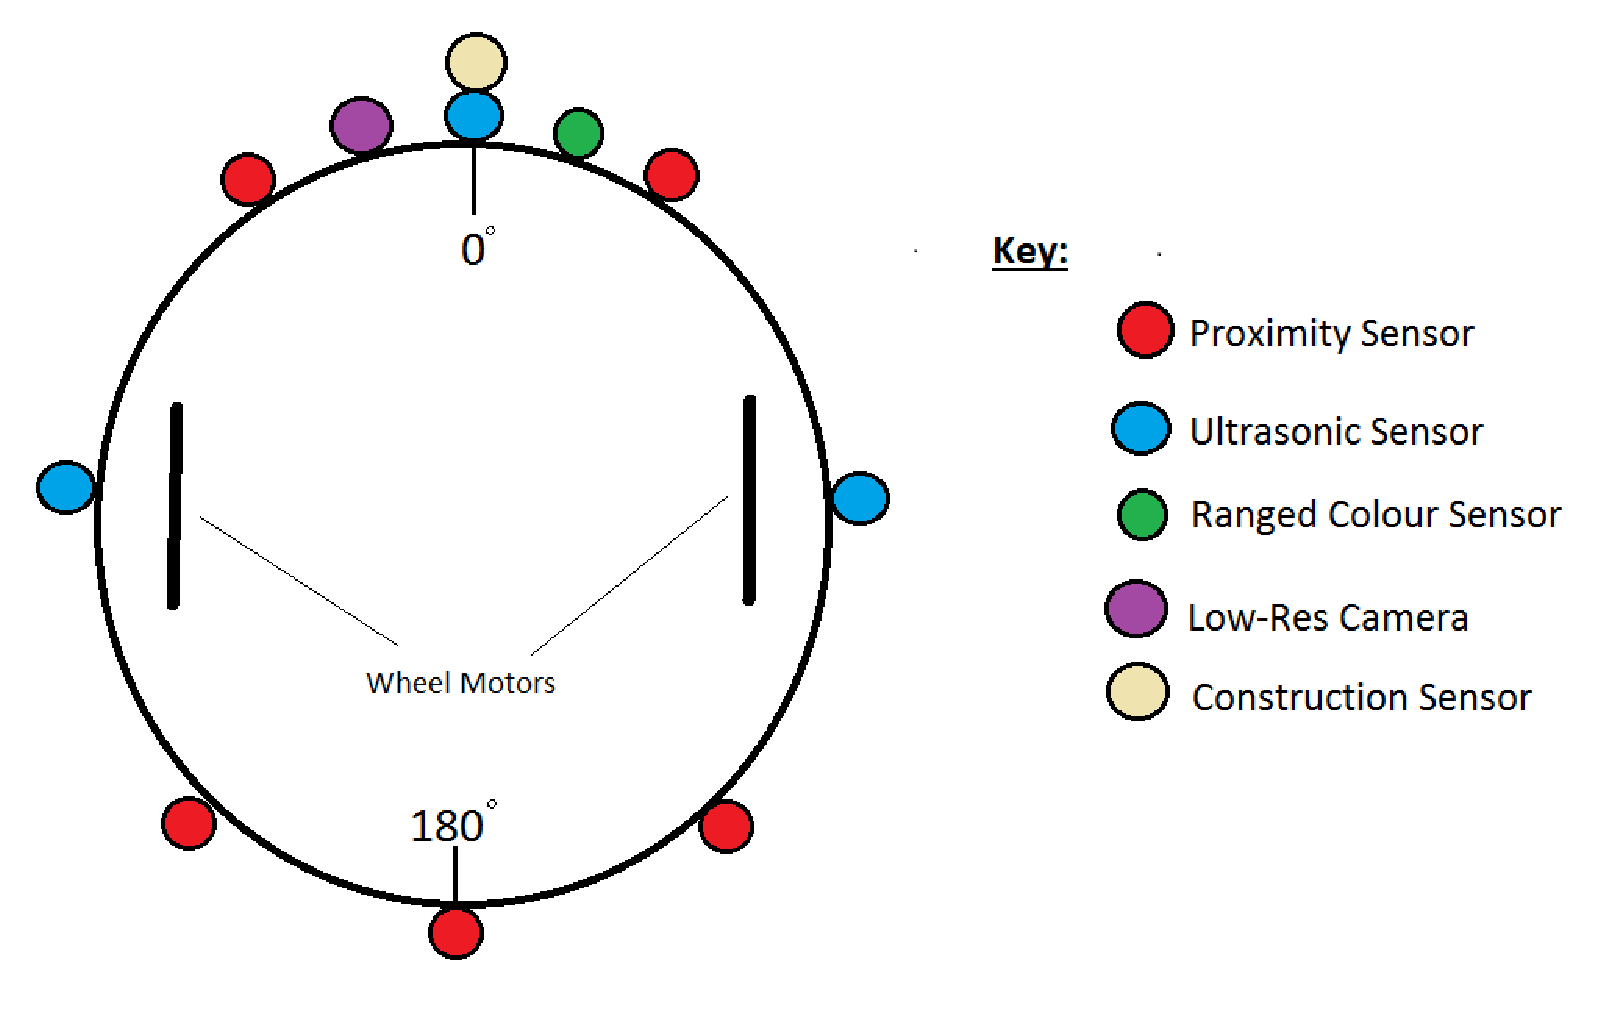
\includegraphics[width=\textwidth]{Morphology.eps}
    \end{minipage}
    \centering
    \begin{minipage}{0.60\textwidth}
       	\centering
        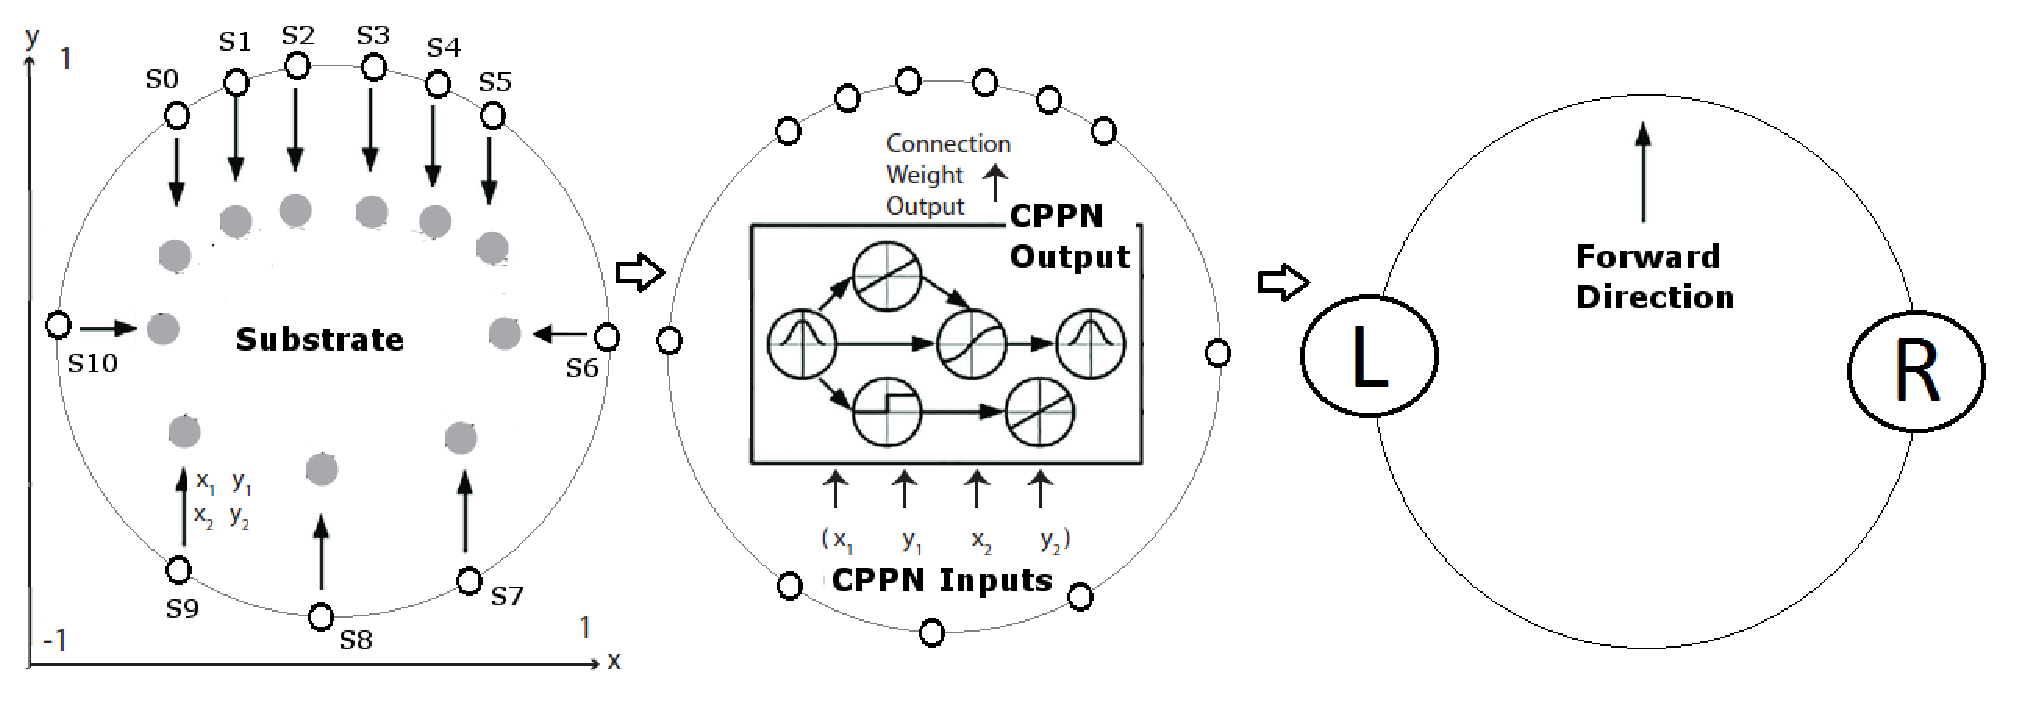
\includegraphics[width=\textwidth]{ANN_Config3.eps}
    \end{minipage}
    \caption{\textit{Left (color):} Robot morphology $1$, with relative positions of various sensors on the robot.
    \textit{Right (gray-scale):} ANN Topology as it relates to robot morphology $1$: $11$ Sensory inputs [S0, S10].  Sensory inputs connect to a hidden
    layer (left).  Connection weight values between two nodes ($x_{1}$, $y_{1}$, $x_{2}$, $y_{2}$) are evolved by querying the CPPN (center) with x, y
    values in the range [-1, 1] (axis shown).  The hidden layer is fully connected to all inputs and outputs (connectivity not depicted).
    Motor outputs (right)
    \textit{L} and \textit{R} determine the speed of the left and right wheels, respectively, and thus a robot's speed and direction.}\label{fig:ann}
\end{figure*}


\begin{table*} [t]
	\renewcommand{\arraystretch}{1.50}
	\caption{Sensory configuration (number of sensors) for each morphology.}\label{tab:morphConfigs}
	\centering
	\begin{tabular}{| c | c | c | c | c | c |}
		\hline
\textbf{Morphology ID} & \textbf{Proximity Sensors} & \textbf{Ultrasonic Sensors} & \textbf{Color Ranged Sensors} & \textbf{Low-Resolution Camera} & 	 \textbf{Construction Zone Sensors} \\
%                       &   Sensors     &   Sensors          &  Sensors         &   Camera          &   Zone Sensors \\
		\hline
		\textbf{1}               &	5 	 	    & 	3  	             &	1               &	1                &	1   \\
		\textbf{2}               &	4 	 	    &	1		         &	1	            &	1                &	1   \\
		\textbf{3}               &	0 	        &	0				 &	1			    &	1                &	1    \\
		\textbf{4}               &	2 		 	&	0	     		 &	1		        &	1                &	1    \\
		\textbf{5}               &	2  	        & 	2				 &  1               &	1                &	1    \\
		\hline
	\end{tabular}
\end{table*}

Objective
Morph_1
20 Repeats
100 Generations
5 Fitness Function Runs
Morph_2
20 Repeats
100 Generations
5 Fitness Function Runs
Morph_3
20 Repeats
100 Generations
5 Fitness Function Runs
Novelty
Morph_1
20 Repeats
100 Generations
5 Fitness Function Runs
Morph_2
20 Repeats
100 Generations
5 Fitness Function Runs
Morph_3
20 Repeats
100 Generations
5 Fitness Function Runs
Hybrid
Morph_1
20 Repeats
100 Generations
5 Fitness Function Runs
Morph_2
20 Repeats
100 Generations
5 Fitness Function Runs
Morph_3
20 Repeats
100 Generations
5 Fitness Function Runs



\begin{figure}[t]
	\centering
	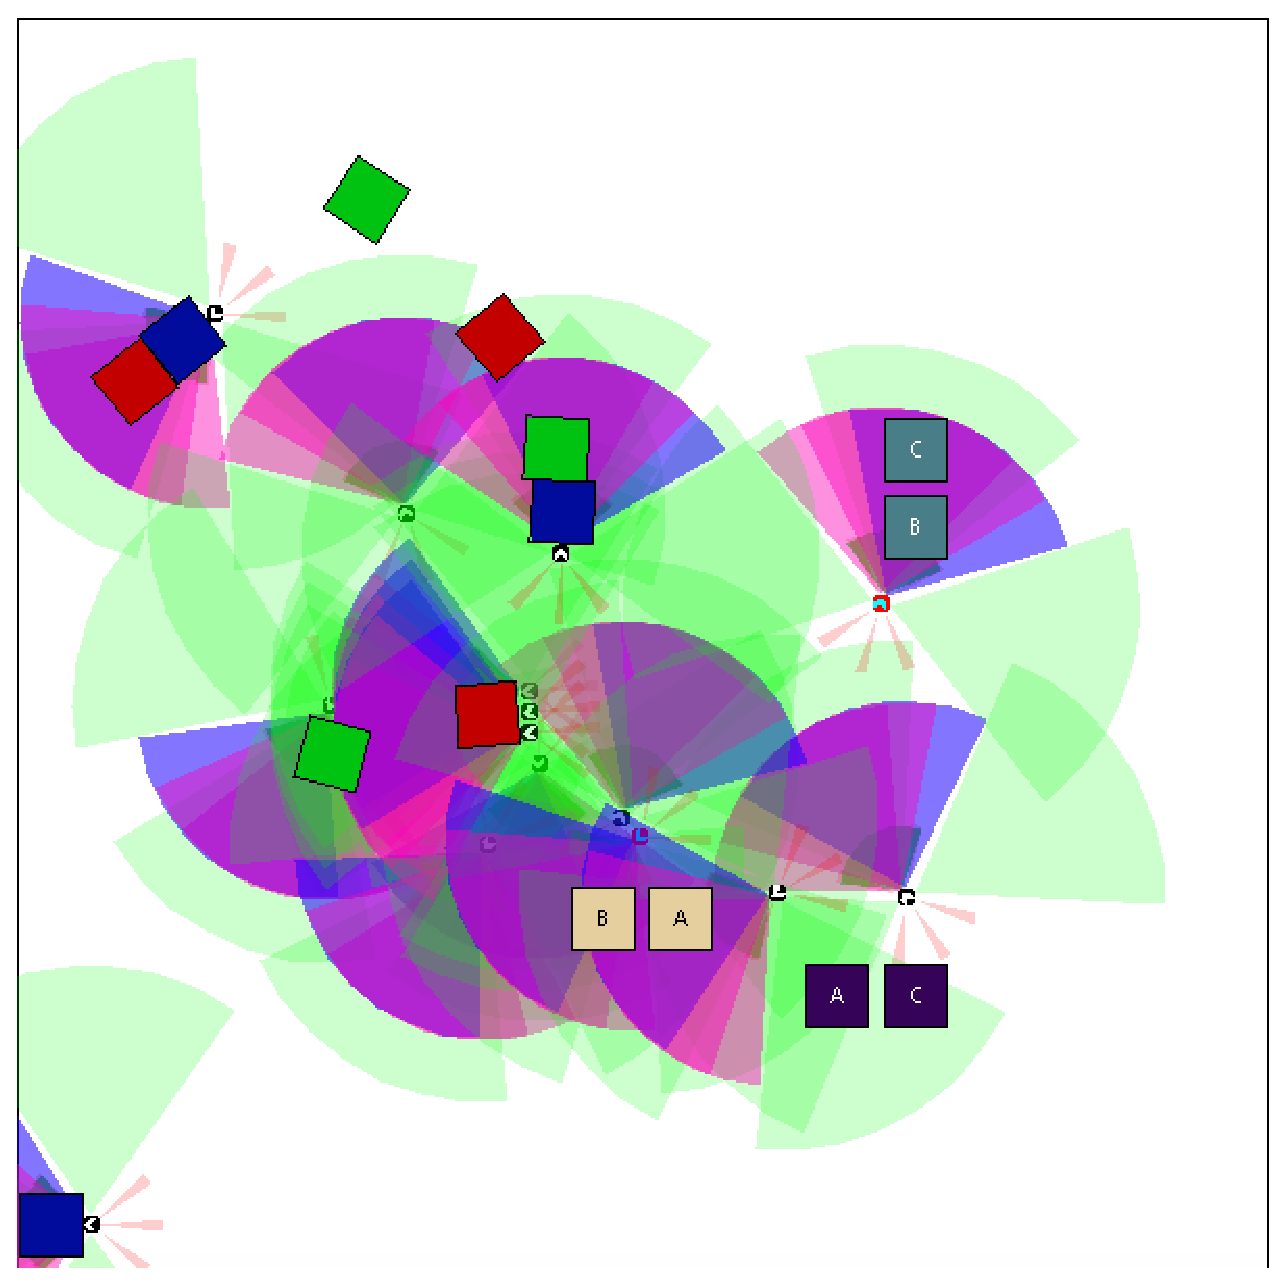
\includegraphics[width=0.40\textwidth]{TaskEnv.eps}
\caption{Example of the simulation environment.  Robots search for randomly distributed
type A, B, and C blocks (blue, green and red, respectively).  Other colored and labeled
blocks indicate those already connected in construction zones.
Different coloured semi-circles emanating from each
robot represent the field of view of currently active different sensor types (table \ref{tab:simParameters}).}\label{fig:taskEnv}
\end{figure}

\begin{figure}[t]
	\centering
	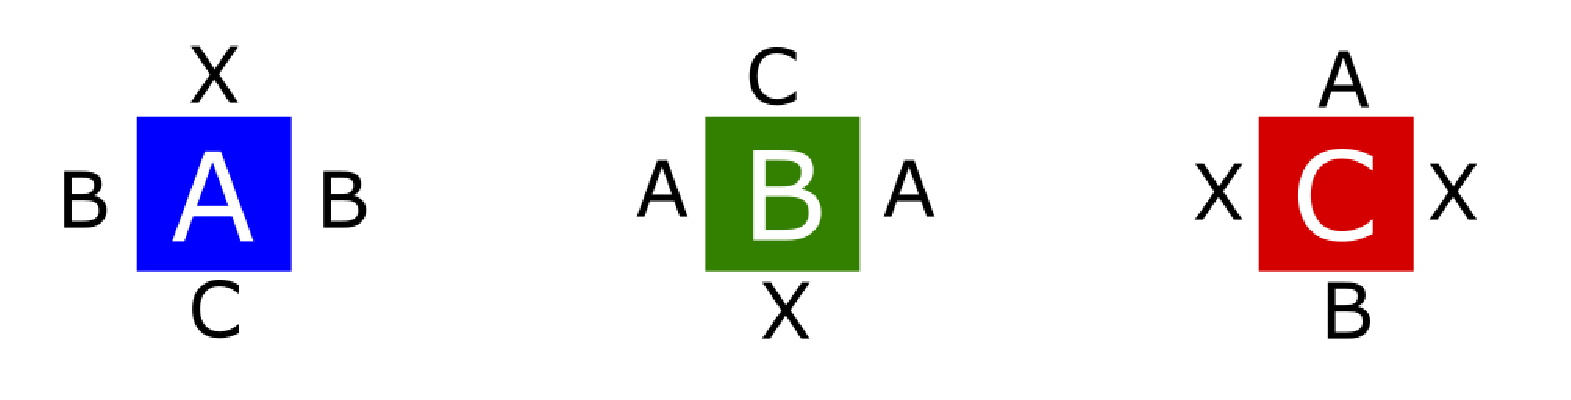
\includegraphics[width=0.5\textwidth]{ConstructionSchema.eps}
	\caption{Task level 3 construction schema: \textit{A}, \textit{B}, and \textit{C} are the block types.  The label on
each side of each block type indicates what block type can be connected to this side.  An \textit{X} label indicates
that no block can be connected.}\label{fig:constructionSchema}
\end{figure}



\begin{table}
	\renewcommand{\arraystretch}{1.30}
	\caption{Experiment, Neuro-evolution and Sensor Parameters}\label{tab:simParameters}
	\centering
	\begin{tabular}{llc}
		\hline
		Generations	                                           & 100	\\
		Sensors per robot                                      & 11, 8, 4, 6, random \\	
		Evaluations per genotype                               & 5  \\
		Experiment runs                                        & 20 \\
		Environment length, width                              & 20 \\
        Max Distance (Robot movement per iteration)            & 1.0 \\
        Team size                                              & 15 \\
        Team Lifetime (Simulation iterations)                  & 1000 \\	
        Lifetimes per generation                               & 5 \\
        Type A blocks (1 robot to push)                        & 15 \\
        Type B blocks (2 robots to push)                       & 15 \\
        Type C blocks (3 robots to push)                       & 15 \\
		\hline
		\multirow{4}{*}{Mutation rate} & Add neuron            & 0.25 \\
		& Add connection                                       & 0.008  \\
		& Remove connection                                    & 0.002 \\
		& Weight                                               & 0.1  \\
		Population size                                        & 150 \\
		Survival rate                                          & 0.3 \\
		Crossover proportion                                   & 0.5 \\
		Elitism proportion                                     & 0.1 \\
		CPPN topology                                          & Feed-forward           \\
		CPPN inputs                                            & Position, delta, angle \\
		\hline
		Sensor                                                 & Range     & FOV \\
		\hline
		Proximity Sensor		                               & 	1.0	   &  0.2  \\
		Ultrasonic Sensor		                               &	4.0    &  1.2  \\
		Ranged Colour Sensor	                               &	3.0	   &  1.5 \\
		Low-Res Camera			                               & 	3.0	   &  1.5 \\
		Colour Proximity Sensor                                & 	3.0	   &  3.0 \\
		\hline
	\end{tabular}
\end{table}

\begin{table}[t]
	\renewcommand{\arraystretch}{1.30}
	\caption{Task Complexity. Note: Task level 3 includes a construction schema (figure \ref{fig:constructionSchema}).}\label{tab:taskComplexity}
	\centering
	\begin{tabular}{lccc}
		\hline
		Construction Task Complexity                               & Level 1     & Level 2    & Level 3   \\
		\hline
		Type A blocks (1 robot to push)	                           & 	15	     & 5          & 5  \\
		Type B blocks (2 robots to push)		                   &	0 	     & 5          & 5  \\
		Type C blocks (3 robots to push)	                       &  	0	     & 5          & 5  \\
		Construction schema                                        &   No        & No         &	Yes \\
\hline
	\end{tabular}
\end{table}



\begin{figure*}[t]
	\begin{minipage}{0.5\textwidth}
		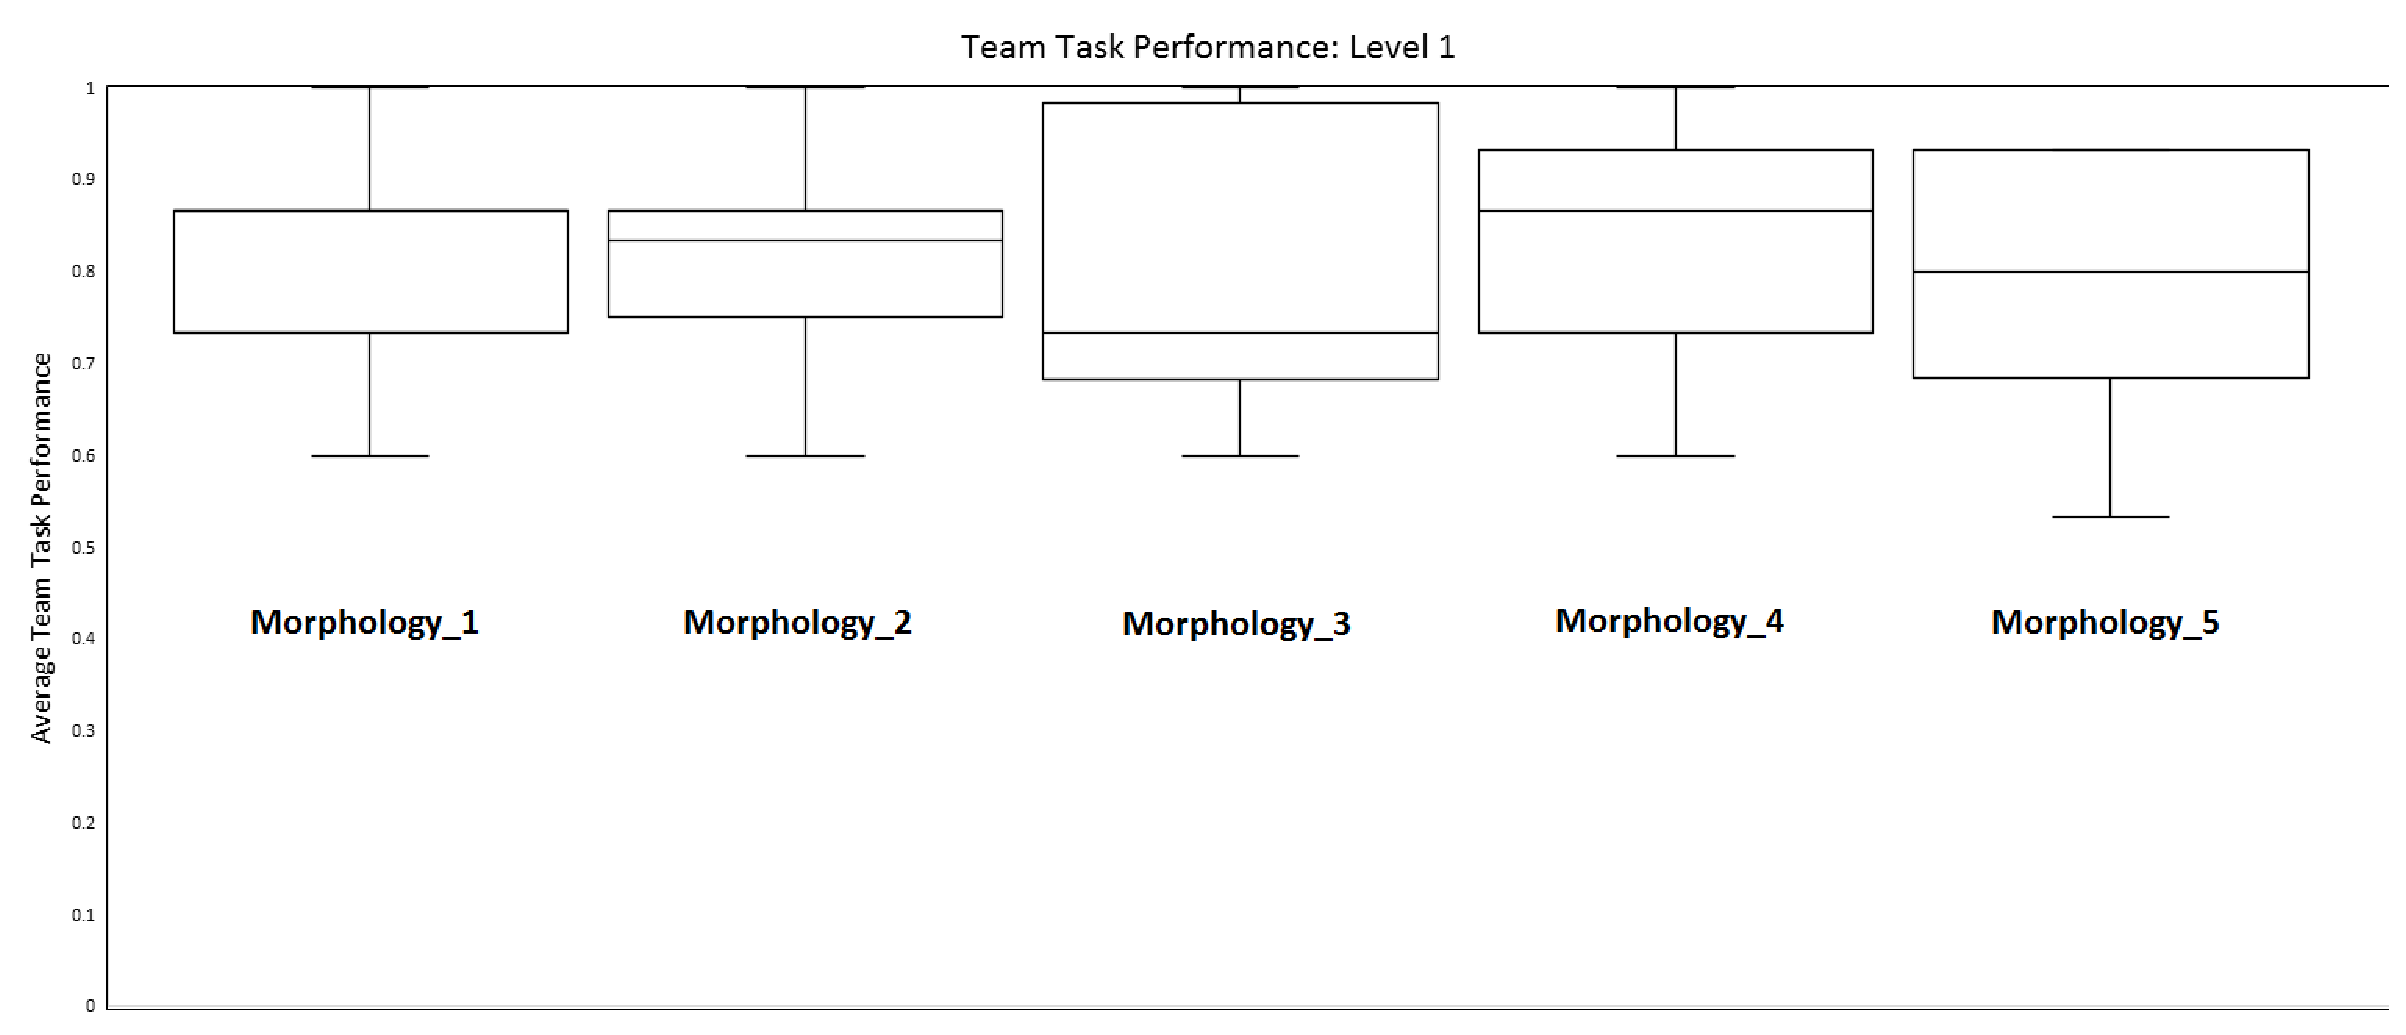
\includegraphics[width=\textwidth]{Evo_BoxPlot_Level1.eps}
	\end{minipage}
	\begin{minipage}{0.5\textwidth}
		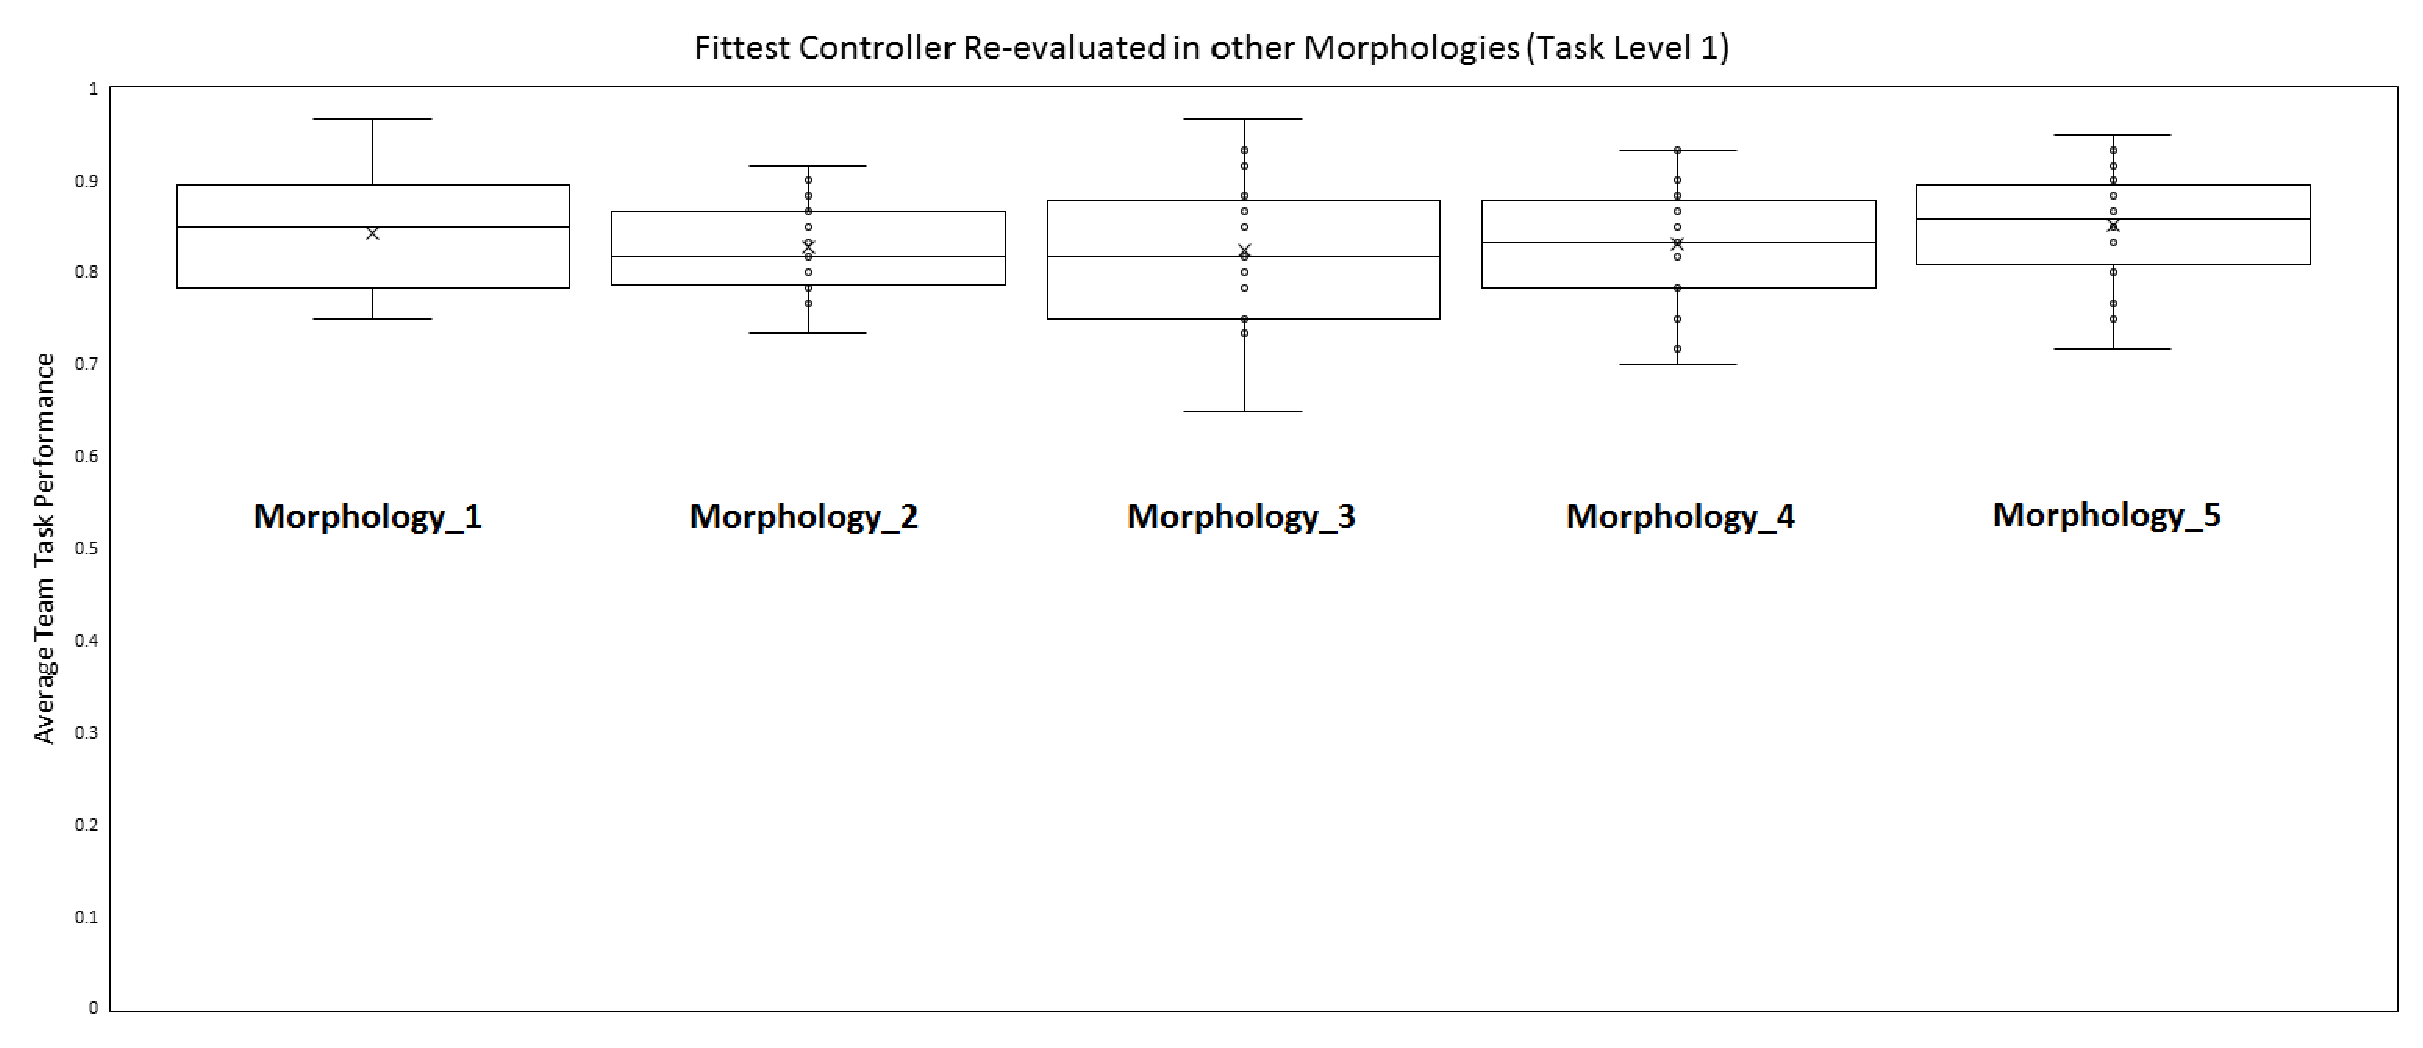
\includegraphics[width=\textwidth]{Level1_ReEval.eps}
	\end{minipage}
\caption{\textit{Left column:} Average team task performance for controller evolution (\textit{task level 1})
given morphologies $1-5$ (depicted from left to right).
\textit{Right column:} Average task performance given the fittest controller evolved
for each successive morphology ($1-5$, shown left to right) re-evaluated in all other morphologies.
For example: Left-most plot is average task performance of fittest controller evolved for
morphology $1$, re-evaluated in morphologies $2-5$.  Right-most plot is the average task performance
of fittest controller evolved for morphology $5$, re-evaluated in morphologies $1-4$.}\label{fig:level1results}
\end{figure*}

\begin{figure*}[t]
	\begin{minipage}{0.5\textwidth}
		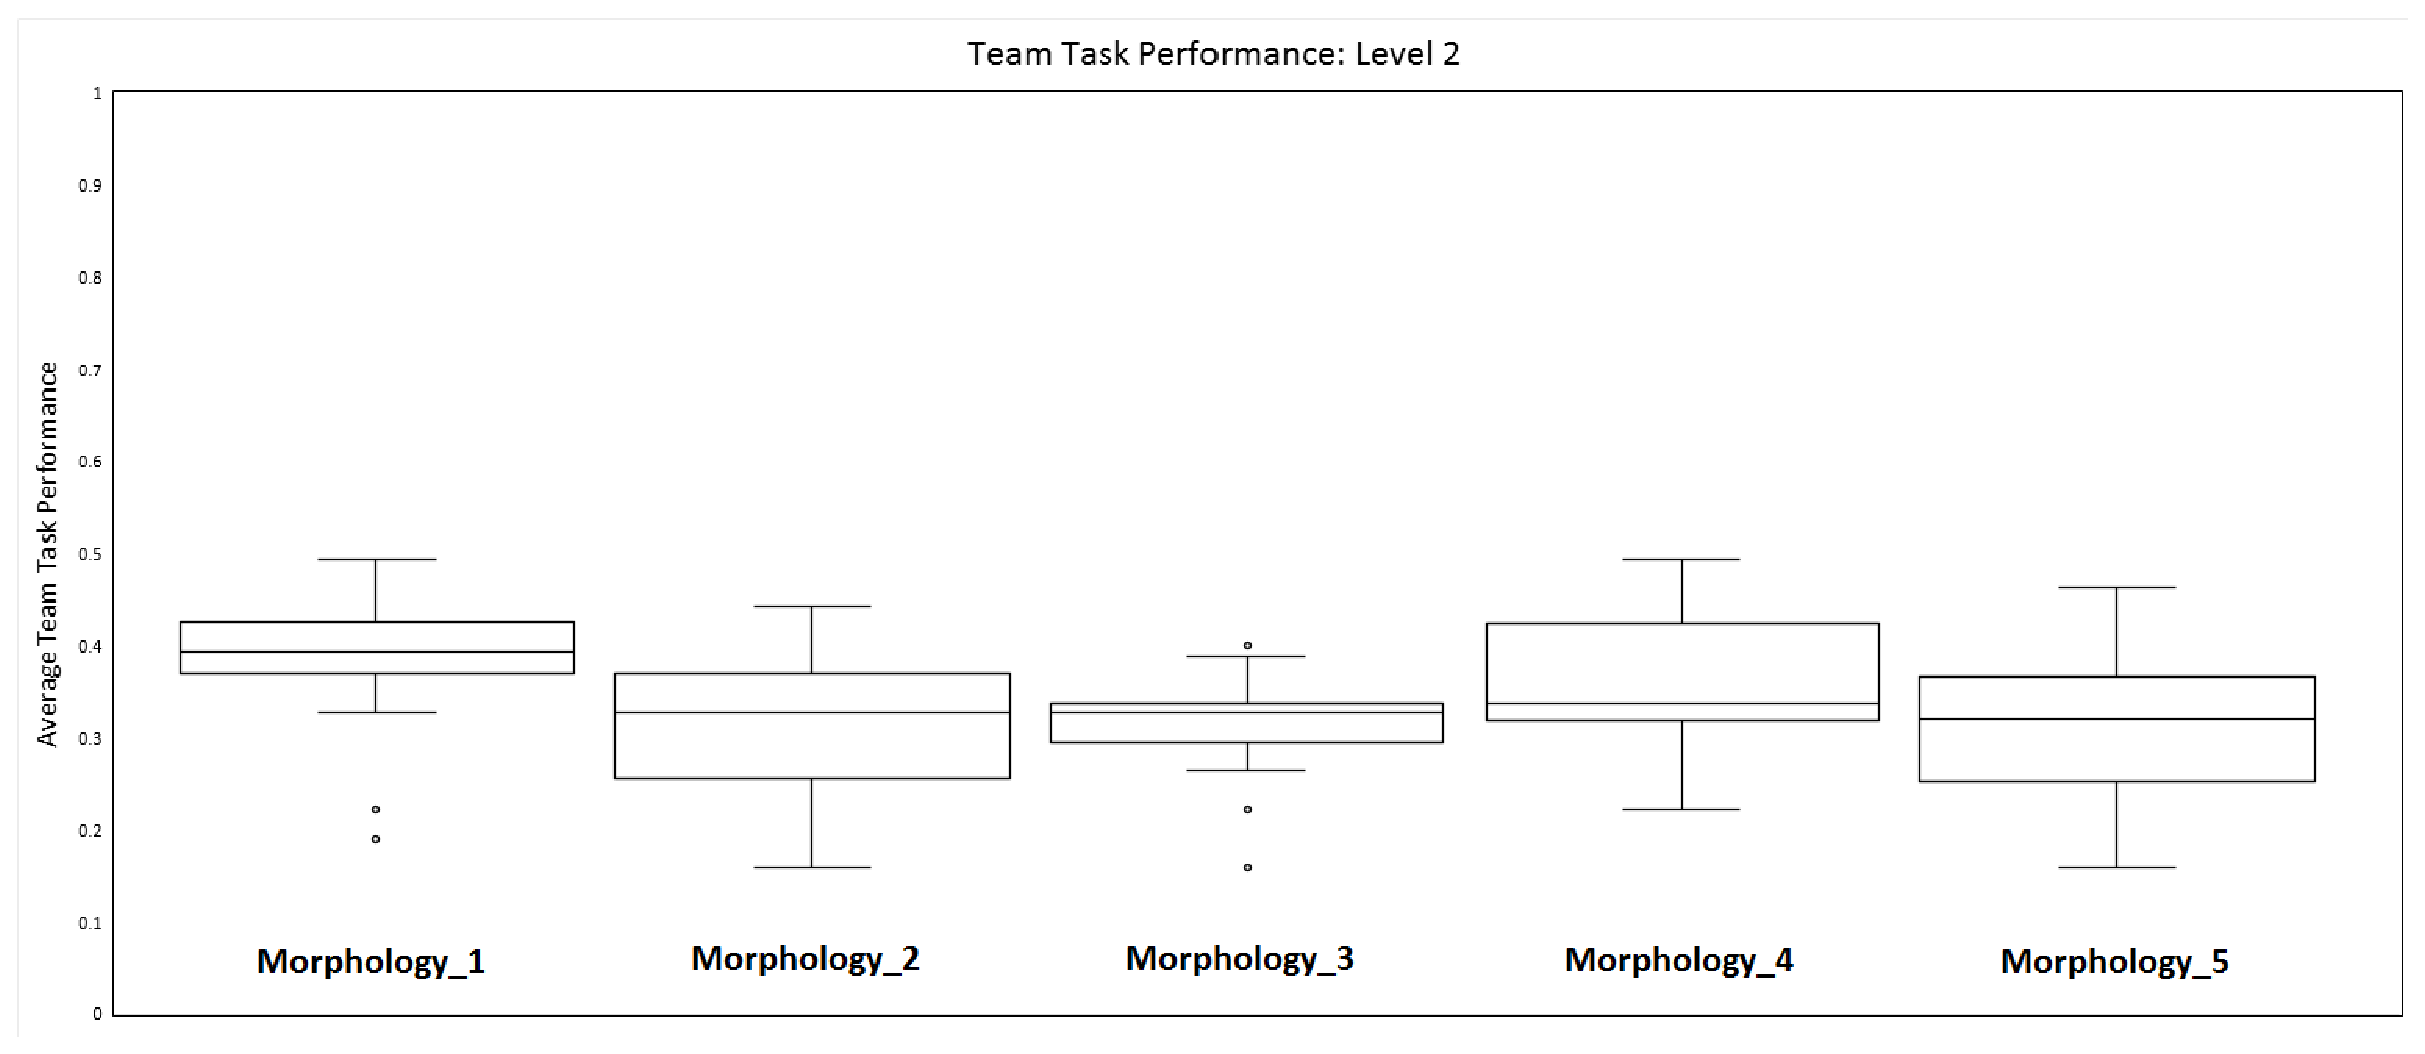
\includegraphics[width=\textwidth]{Evo_BoxPlot_Level2.eps}
	\end{minipage}
	\begin{minipage}{0.5\textwidth}
		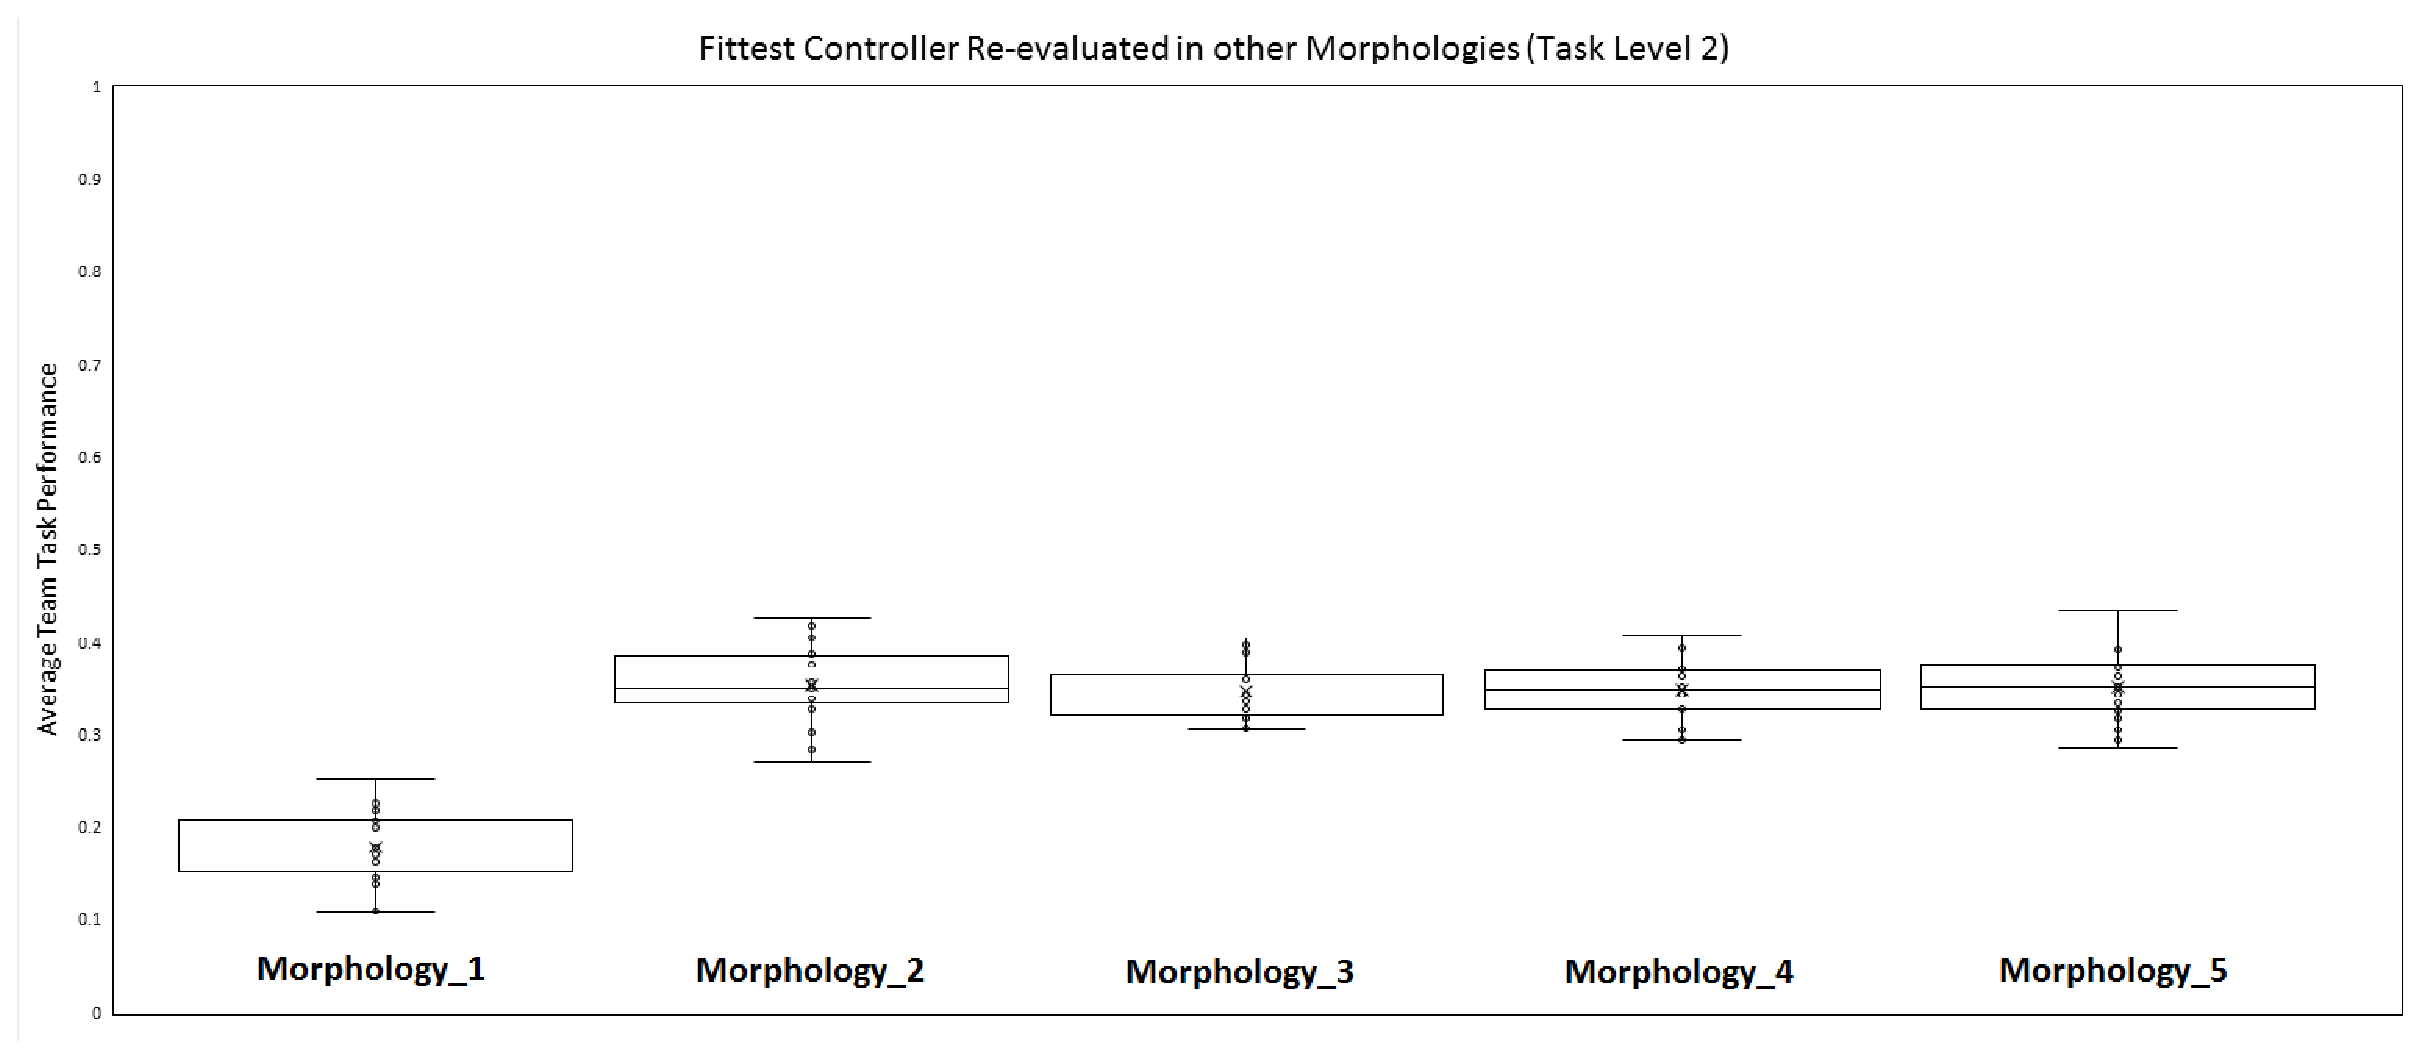
\includegraphics[width=\textwidth]{Level2_ReEval.eps}
	\end{minipage}
\caption{\textit{Left column:} Average team task performance for controller evolution (\textit{task level 1})
given morphologies $1-5$ (depicted from left to right).
\textit{Right column:} Average task performance given the fittest controller evolved
for each successive morphology ($1-5$, shown left to right) re-evaluated in all other morphologies.
For example: Left-most plot is average task performance of fittest controller evolved for
morphology $1$, re-evaluated in morphologies $2-5$.  Right-most plot is the average task performance
of fittest controller evolved for morphology $5$, re-evaluated in morphologies $1-4$.}\label{fig:level2results}
\end{figure*}

\begin{figure*}[t]
	\begin{minipage}{0.5\textwidth}
		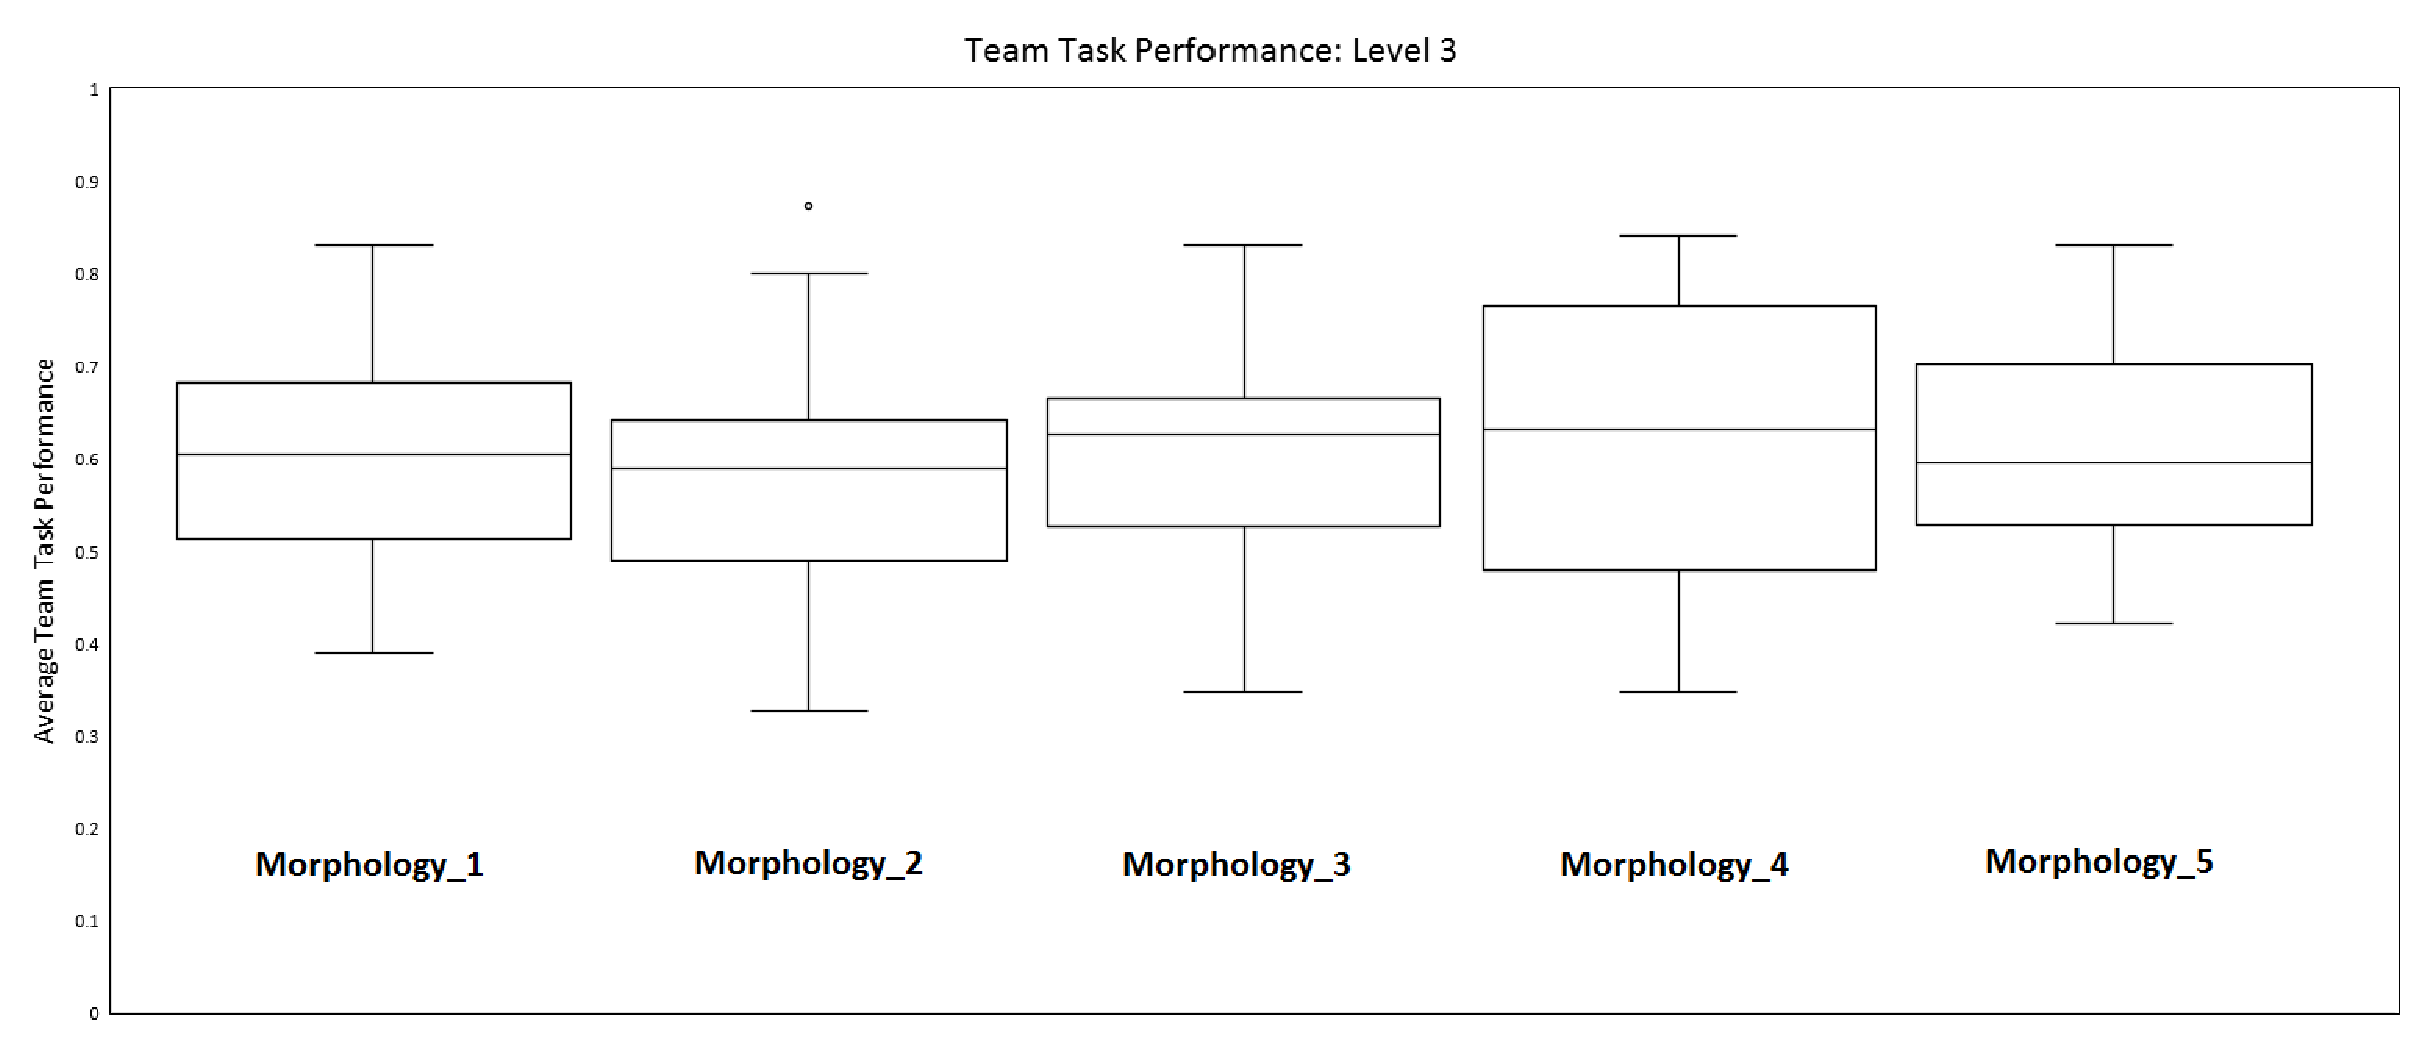
\includegraphics[width=\textwidth]{Evo_BoxPlot_Level3.eps}
	\end{minipage}
	\begin{minipage}{0.5\textwidth}
		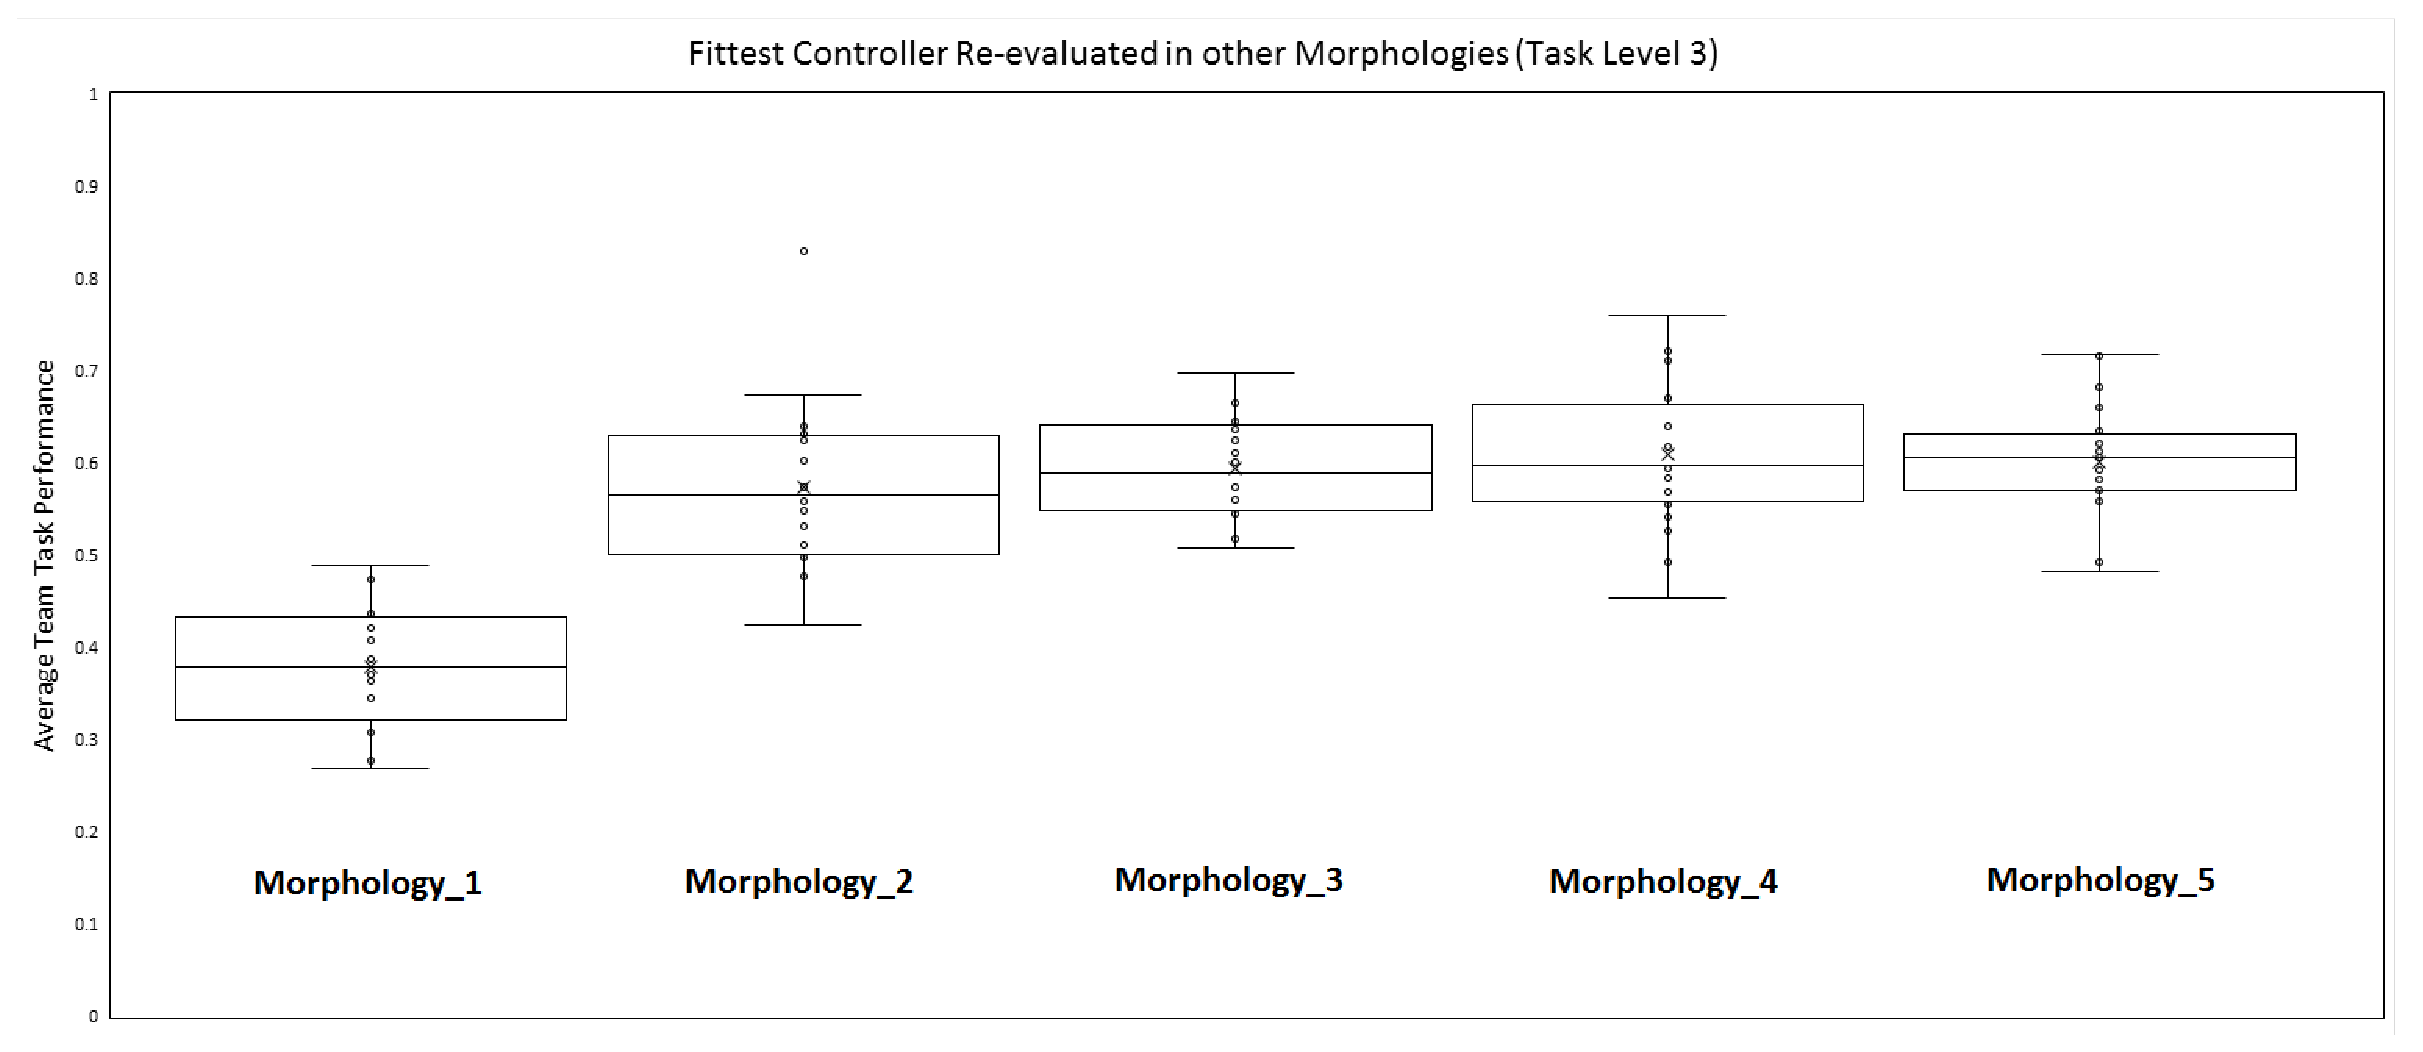
\includegraphics[width=\textwidth]{Level3_ReEval.eps}
	\end{minipage}
\caption{\textit{Left column:} Average team task performance for controller evolution (\textit{task level 1})
given morphologies $1-5$ (depicted from left to right).
\textit{Right column:} Average task performance given the fittest controller evolved
for each successive morphology ($1-5$, shown left to right) re-evaluated in all other morphologies.
For example: Left-most plot is average task performance of fittest controller evolved for
morphology $1$, re-evaluated in morphologies $2-5$.  Right-most plot is the average task performance
of fittest controller evolved for morphology $5$, re-evaluated in morphologies $1-4$.}\label{fig:level3results}
\end{figure*}

%\begin{table}[t]
%	\renewcommand{\arraystretch}{1.30}
%	\caption{Two-way ANOVA: Impact of sensor configuration and task complexity on team performance - Task level 1.}\label{tab:anovaL1}
%	\centering
%	\begin{tabular}{lrrrrr}
%				     &     Df  & SS & MS & F & p \\
%    	\hline
%        Complexity    			&   2  & 27.88  & 13.94 &   1187.36 & \(1.6 \times 10^{-181}\)\\
%        Morphology   	 		&   7  & 3.68   & 0.53 &   44.8 & \(3.9 \times 10^{-48}\)		\\
%        Complexity:Morphology 	&   14 & 2.28   & 0.16 &   13.86 &  \(1.29 \times 10^{-27}\)	\\
%        Residuals     			&   456& 39.19  & 0.12 &          &               \\
%        \hline
%	\end{tabular}
%\end{table}

%\begin{table}[t]
%	\renewcommand{\arraystretch}{1.30}
%	\caption{Two-way ANOVA: Impact of sensor configuration and task complexity on team performance - Task level 2.}\label{tab:anovaL2}
%	\centering
%	\begin{tabular}{lrrrrr}
%								& Df  & SS & MS & F & p \\
%		\hline
%		Complexity    			&   2 & 17.81 & 8.92 &   649.21 & \(3.8 \times 10^{-134}\)\\
%		Morphology   	 		&   7 & 0.19 & 0.03 &   1.98 &  0.06		\\
%		Complexity:Morphology 	&   14 & 0.15 & 0.01 &   0.79 &  0.68	\\
%		Residuals     			& 456 & 6.26 & 0.01 &          &               \\
%		\hline
%	\end{tabular}
%\end{table}

%\begin{table}[t]
%	\renewcommand{\arraystretch}{1.30}
%	\caption{Two-way ANOVA: Impact of sensor configuration and task complexity on team performance - Task level 3.}\label{tab:anovaL3}
%	\centering
%	\begin{tabular}{lrrrrr}
%								& Df  & SS & MS & F & p \\
%		\hline
%		Complexity    			&   2 & 24.67 & 12.34 &   920.91 & \(7.3 \times 10^{-161}\)\\
%		Morphology   	 		&   7 & 0.25 & 0.04 &   2.69 &  0.01 \\
%		Complexity:Morphology 	&   14 & 1.49 & 0.11 &   7.94 &  \(3.41 \times 10^{-15}\)	\\
%		Residuals     			& 456 & 6.11 & 0.01 &          &         \\
%		\hline
%	\end{tabular}
%\end{table}

\section{Results \& Discussion}

For each controller evolution experiment, the average maximum task performance
of controllers evolved for a given morphology and level of task complexity, was recorded.
Specifically, this task performance was calculated by running the absolute fittest controller
evolved after $20$ evolutionary runs (for a given a morphology and task level),
in the same morphology over $20$ non-evolutionary runs.
This is presented in figures \ref{fig:level1results}, \ref{fig:level2results} and \ref{fig:level3results}
(left column), where controllers were evolved given morphologies $1$-$5$ (table \ref{tab:morphConfigs}).
In figures \ref{fig:level1results}, \ref{fig:level2results} and \ref{fig:level3results} (left column),
these results are presented from left to right.
For example, average task performance results for morphology $1$ are plotted on the left-most side
and average task performance results for morphology $5$ are plotted on the right-most side.

For each re-evaluation experiment, the fittest controller evolved for a given morphology and task complexity
level was re-evaluated in all other morphologies (for the same level of task complexity), and an
average task performance computed over $20$ runs.
These morphological re-evaluation results are presented in figures \ref{fig:level1results}, \ref{fig:level2results}
and \ref{fig:level3results} (right column).
Each of the five plots (from left to right) in each figure corresponds to the fittest controller evolved for each of the
five morphologies and re-evaluated in all other morphologies.  For example, the left-most plot presents
the average task performance of the fittest controller evolved in morphology $1$ and re-evaluated on morphologies $2-5$.
Where as, the right-most plot presents the average task performance of the fittest controller evolved given morphology $5$
(as the initial sensory configuration) and re-evaluated on morphologies $1-4$.

To gauge the impact of a given team morphology (table \ref{tab:morphConfigs})
in company with a given level of task complexity (table \ref{tab:taskComplexity}),
the \textit{t-test} \cite{FlanneryTeukolsky1986} ($p < 0.05$),
was applied in pair-wise comparisons between sets of controller evolution
results\footnote{Statistical test results for pair-wise comparisons for the fittest evolved controllers
(for a given morphology) tested in each other morphology (individually) is online at:
\url{https://github.com/not-my-name/SSCI_Paper_Appendix}}
(figures \ref{fig:level1results}, \ref{fig:level2results} and \ref{fig:level3results}, left column).
Within each given level of task complexity, no statistically significant difference was found between
controllers evolved given morphologies $1-5$ (controller evolution experiments $1-5$).
Controller evolution experiments $1-4$ were those implementing controller evolution in fixed sensory
configurations (morphologies $1-4$).  Where as, controller evolution experiment $5$ used morphology $5$
as the initial sensory configuration and subsequently co-adapted behavior (controller) and morphology
(complement of sensors).
The lack of statistical difference between controllers evolved given morphologies $1-4$ (table \ref{tab:morphConfigs})
indicates that these sensory configurations were not sufficiently different so as to result in
significantly different average maximum task performances.
Also, the lack of any significant difference between the average maximum task performance of controllers
evolved given morphologies $1-4$ and behavior-morphology co-adaptation (starting with morphology $5$),
supports previous results demonstrating that behavior-morphology co-adaptation
yields at least comparable task performance benefits (compared to fixed morphology controller evolution)
in collective behavior tasks \cite{HewlandNitschke2015}.

However, to address this study's main objective it was necessary to ascertain the morphological robustness
of the fittest controller evolved in each morphology when re-evaluated in all other morphologies.
To gauge the morphological robustness of the fittest controllers evolved for a given morphology ($1-5$),
and a given task complexity, we applied the t-test in pair-wise comparisons of two result
data sets.  First, the average maximum task performances yielded by controller evolution in morphologies
$1-5$ and second, the average maximum task performances yielded from re-evaluating the fittest controller
evolved for a given morphology in all other morphologies (section \ref{subsec:expDesign}).
%Thus, we also used two-way ANOVA tests to measure the impact of task complexity and re-evaluating the fittest
%controller evolved for each morphology on all morphologies (in comparison to controller evolution results).

Statistical test results indicated no significant difference (with one exception) between average task performance results
yielded by controller evolution and morphological re-evaluation experiments for all task complexity levels.
Specifically, the average maximum task performance yielded by controllers evolved given morphologies $2$-$5$
(figures \ref{fig:level1results}, \ref{fig:level2results}, \ref{fig:level3results}, left column) was not
significantly lower than the average task performance yielded by the fittest controllers
(evolved in morphologies $1-5$), and then re-evaluated on other morphologies
(figures \ref{fig:level1results}, \ref{fig:level2results}, \ref{fig:level3results},
right column).  The exception was morphology $1$ in task complexity levels $2$ and $3$.
In these tasks, the fittest controller evolved for morphology $1$, yielded a significantly higher average
task performance than that yielded when this fittest controller was re-evaluated in
morphologies $2-5$.
%Statistical test results are summarized in tables \ref{tab:anovaL1}, \ref{tab:anovaL2}
%and \ref{tab:anovaL3} for task complexity levels $1$, $2$ and $3$, respectively,
%and include performance results comparisons between controller evolution and
%morphological re-evaluation experiments with respect to task complexity and morphology.

Hence, these results indicate that controllers evolved by HyperNEAT for a given morphology
(table \ref{tab:morphConfigs}), overall have the capacity to continue to effectively operate
when transferred to other morphologies.
This result was found to hold for all four of the five morphologies that controllers were evolved for,
and for all levels of task complexity tested (table \ref{tab:taskComplexity}).
%thus demonstrating the morphological robustness of HyperNEAT evolved controllers.

The efficacy of HyperNEAT for evolving morphologically robust controllers is further supported
by the controller evolution experiments that used morphology $5$ (section \ref{sec:experiments}).
In this case, the number of sensors was adapted meaning that team behavior and
morphology were co-adapted.
Specifically, these controller evolution experiments began with the sensory configuration of
morphology $5$ (table \ref{tab:morphConfigs}) and enabled and disabled sensor connections to
better couple morphology with the evolved controller.  Hence, the fittest
controller evolved in this case often corresponded to a sensory configuration
dissimilar to morphology $5$ (the initial sensory configuration).
Results indicated that the fittest controller evolved for morphology $5$, when re-evaluated in
other morphologies, yielded an average task performance that was statistically comparable to
the average task performance yielded by controller evolution given morphology $5$.
This result was observed for all three task complexity levels
(figures \ref{fig:level1results}, \ref{fig:level2results}, and \ref{fig:level3results}, right column).

Thus, controllers evolved for fixed morphologies ($1-4$, table \ref{tab:morphConfigs}), were
found to be \textit{morphologically robust}, as there was no significant difference in average maximum
task performance when the fittest controller (evolved for morphology $1-4$), was re-evaluated in other
morphologies.
Furthermore, the fittest controller evolved for an adaptive morphology ($5$, table \ref{tab:morphConfigs}),
was similarly found to be morphologically robust, given that the average maximum task performance
yielded when this fittest controller was re-evaluated in other morphologies ($1-4$), was comparable to
the average maximum task performance yielded from morphology $5$ controller evolution experiment.
This is theorized to be a result of the complexity of co-adapting effective controller-morphology
couplings \cite{PfeiferBongard2006} within limited periods of artificial evolution ($100$ generations in these experiments,
table \ref{tab:simParameters}), offset by the transference of evolved
\textit{connectivity patterns} \cite{GauciStanley2010} as functional controllers across varying
robot morphologies  \cite{RisiStanley2013}.
Such connectivity patterns encode behaviors that do not rely upon specific sensory-motor mappings in
controllers and thus do not necessitate specific task environment configurations,
such as specific numbers of agents or objects.
This in turn facilitates the transfer of controllers across varying team morphologies
\cite{verbancsics_evolving_2010}, \cite{DidiNitschke2016SSCI}, \cite{DidiNitschke2016}.
%a benefit of HyperNEAT elucidated from such collective behavior transfer research was found to be its capability
%to evolve connectivity patterns between the sensory-motor layers of agent controllers
%that are broadly applicable to collective behavior tasks of varying complexity.
%versus adaptive morphologies had no significant impact on the
%morphological robustness of HyperNEAT evolved controllers (gauged in terms of average team task performance)
%for all morphologies tested.  %This result was observed for all levels of task complexity tested.

These results are corroborated by related work \cite{RisiStanley2013}, \cite{WatsonNitschke2015SSCI},
and contribute further empirical evidence that HyperNEAT yields significant benefits in
evolving robot controllers that effectively operate in other morphologies.
That is, this study further demonstrated HyperNEAT's capability to exploit geometric properties
such as regularity, repetition and symmetry in robot morphology and environment \cite{StanleyDAmbrosioGauci2009},
where such modularity and geometric properties are encoded in evolved connectivity patterns.
This is prevalent in this study, as the configuration of sensors on each robot's periphery was
symmetrical for all morphologies tested (section \ref{sec:embodiment}).
Also, the collective construction task required that blocks be connected together in a repeated manner in a symmetrical bounded
simulation environment ($20$x$20$ units, table \ref{tab:simParameters}).
The capability of HyperNEAT evolved controllers to operate in different morphologies is further
supported by other research \cite{verbancsics_evolving_2010}
demonstrating that evolved indirect sensory-motor mappings can
encapsulate effective behaviors with relatively few task environment and robot
geometric relationships, such as desired positions and angles between robots and different object types.

The efficacy of HyperNEAT for evolving morphologically robust controllers for collective behavior
tasks of varying complexity is also supported by related research in \textit{multi-agent policy transfer}
\cite{verbancsics_evolving_2010}, \cite{DidiNitschke2016SSCI}, \cite{DidiNitschke2016}.
Policy transfer methods facilitate the transfer of behaviors across tasks of increasing
complexity or between dissimilar tasks.  Such studies have demonstrated that HyperNEAT is an effective
method for evolving behaviors in one collective behavior task and then transferring the evolved behavior
to a related but more complex task (for example, where robots have more complex sensory-motor configurations
to process increased task complexity) with relatively little loss in average team task performance.
%That is, HyperNEAT evolves CPPNs representing controllers of varying complexity with their own symmetries
%and regularities which are able to effectively exploit varyingly complex robot (agent) sensory-motor configurations.
%This in turn, often significantly boosts the efficacy of evolved collective behaviors \cite{DAmbrosio2013}.

However, we hypothesize that the morphological robustness of HyperNEAT evolved controllers demonstrated across all
morphologies tested (table \ref{tab:morphConfigs}) and all levels of task complexity
(table \ref{tab:taskComplexity}) was facilitated by the use of morphologically and behaviorally homogenous teams.
Specifically, one controller was evolved for all robots in a team and all robots used the same sensory configuration, meaning
all robots had the same \textit{collective behavior geometry} \cite{DAmbrosioLehmanStanley2010}.
This in turn simplified the transfer of evolved controllers across varying morphologies with no significant degradation
in average task performance.

Hence, overall, this study's results demonstrate that HyperNEAT is an appropriate method for evolving
morphologically robust controllers.  That is, controllers that are fully functional in a range of team morphologies.
In order to ascertain how well HyperNEAT evolved controllers generalize, ongoing research is evaluating
the evolution of morphologically robust behaviors in behaviorally and morphological heterogenous teams
for complex collective behavior tasks that are irregular and without repetition or symmetry.
Furthermore, current research is comparing HyperNEAT to related evolutionary approaches that have demonstrated
controllers able to accomplish multiple disparate tasks in dynamic environments
\cite{IzquierdoTorres2008}, as well as direct encoding neuro-evolution methods such as NEAT \cite{StanleyMiikkulainen2002}.

\section{Conclusions}

This research presented a study on the efficacy of HyperNEAT for evolving \textit{morphologically robust}
behaviors for homogenous robot teams that must solve a collective behavior task of increasing complexity.
That is, the average maximum task performance of behaviors evolved for a given team morphology (robot
sensory configuration) that was then transferred to a different team morphology.
Controllers that did not yield degraded task performance when transferred to another morphology
were considered to be morphologically robust.
The objective was to test and evaluate methods that generate morphological robust behaviors,
where varying morphologies emulated sensor damage or intentional changes to the sensory systems
of robotic teams.

Results indicated that HyperNEAT was appropriate for generating morphologically robust
controllers for a collective construction task of increasing complexity.
This task required robots to cooperatively push blocks such
that they connected together to form structures.
Task complexity was regulated by
the number of robots required to push blocks and a construction schema mandating that specific block types
be connected in specific ways.
These results support the notion that developmental neuro-evolution methods, such as HyperNEAT,
are appropriate for controller evolution in robotics applications where robot teams
must adapt during their lifetime to damage or otherwise must dynamically
adapt their sensory configuration to solve new unforseen tasks.

\bibliographystyle{IEEEtran}
\bibliography{EvoComp}
%\bibliography{IEEEabrv,necc_paper,EvoComp,Dissertation}

\end{document} 